\documentclass[12pt,a4paper]{article}
\usepackage[utf8]{inputenc}
\usepackage[spanish]{babel}
\usepackage{graphicx}
\usepackage{grffile} % Soporte para nombres de archivos de imagen con espacios y caracteres especiales
\usepackage{listings}
\usepackage{hyperref}
\usepackage{geometry}
\usepackage{float}
\usepackage{caption}
\usepackage{tabularx}
\usepackage{booktabs}
\usepackage{tikz}
\usetikzlibrary{shapes.geometric, arrows.meta, positioning}

% Configuración de márgenes
\geometry{top=2.5cm, bottom=2.5cm, left=2.5cm, right=2.5cm}

% Configuración de la ruta de imágenes para Overleaf
\graphicspath{{Entregable 4/}{Entregable 3/}{Entregable 2/}{./}}

% Estilo de enlaces
\hypersetup{
    colorlinks=true,
    linkcolor=blue,
    filecolor=magenta,      
    urlcolor=cyan,
    pdftitle={Trabajo Práctico Integrador -- ARQ-WEB 2026 (Entregables 1, 2, 3 y 4)},
}

\title{\textbf{Trabajo Práctico Integrador -- ARQ-WEB 2026}\\Despliegue, conectividad, seguridad TLS, verificación experimental, resiliencia y observabilidad de una aplicación web}
\author{Sofia Mereles \and Alba Martinez \and Guillermo Gonzalez}
\date{FP-UNA -- 2026}

\begin{document}

\maketitle

\begin{abstract}
El presente informe documenta las Fases 1, 2, 3 y 4 del proyecto integrador de la asignatura Arquitectura Web. En la primera etapa se estableció la línea base de la infraestructura servidor mediante la configuración de un entorno virtualizado en Ubuntu Server en modo puente (\textit{Bridged}), evaluando y seleccionando la plataforma \textbf{BookStack}. En la segunda etapa se llevó a cabo el despliegue del stack LNMP (Linux, Nginx, MariaDB, PHP 8.5-FPM), la ejecución de migraciones y la verificación del servicio HTTP. En la tercera etapa se implementó la capa de seguridad con TLS 1.3 sobre el dominio \texttt{bookstack.local}, la redirección automática HTTPS, la evaluación experimental del rendimiento de la negociación criptográfica, la inspección de cabeceras HTTP/Gzip/Caché, la comparativa de arquitectura entre proxy e interfaz FastCGI, y el análisis de trazas de red mediante \texttt{tcpdump}. Finalmente, en la cuarta etapa se realizó el endurecimiento (\textit{hardening}) del firewall UFW, la auditoría avanzada de cabeceras de seguridad, la simulación de fallos y resiliencia de servicios, pruebas de carga concurrente con \texttt{ab}, la observabilidad en tiempo real con \texttt{htop} y la matriz de pruebas consolidada.
\end{abstract}

\tableofcontents
\newpage

\section{Objetivos, Alcance y Criterios de Aceptación}
El objetivo general es preparar una infraestructura servidor observable y segura, desplegar la aplicación web \textbf{BookStack} y verificar su comportamiento a nivel de red, rendimiento, resiliencia y seguridad.

\begin{itemize}
    \item \textbf{Alcance (Fase 1):} Preparación de la VM (2 vCPU, 4 GB RAM, 20 GB Disco), asignación de IP estática/DHCP en capa 3, configuración de OpenSSH, verificación de conectividad bidireccional y definición del esquema de arquitectura lógica de 3 capas.
    \item \textbf{Alcance (Fase 2):} Instalación del stack LNMP; creación de la base de datos relacional; migración del esquema de BookStack; configuración del servidor virtual en Nginx y validación del flujo HTTP.
    \item \textbf{Alcance (Fase 3):} Configuración de DNS local (\texttt{bookstack.local}); generación de certificado X.509 autofirmado; habilitación de HTTPS (TLS 1.3) con redirección 301; evaluación de latencia con \texttt{curl}; verificación de cabeceras de seguridad, compresión Gzip y políticas de caché (respuestas 304); comparativa técnica Nginx vs. PHP-FPM; y captura/análisis de paquetes con \texttt{tcpdump}.
    \item \textbf{Alcance (Fase 4):} Restricción de la superficie expuesta mediante firewall UFW; auditoría de cabeceras de seguridad HTTP y cookies; validación de fallos de backend (HTTP 502) y persistencia tras reinicio; pruebas de carga concurrente con \texttt{ab}; monitoreo de recursos en vivo (\texttt{htop}); corrección de hallazgos técnicos y consolidación de la matriz de evidencias.
    \item \textbf{Criterios de Aceptación:} Comunicación ICMP sin pérdida de paquetes, TLS 1.3 activo en puerto 443/TCP, redirección 301 desde puerto 80/TCP, cookies de sesión marcadas como \texttt{Secure} e \texttt{HttpOnly}, 0\% de fallos en pruebas de concurrencia de 1.000 peticiones, y autoarranque verificado de servicios tras reinicio completo.
\end{itemize}

\section{Selección de la Aplicación Web}

Para la selección del proyecto se evaluaron dos soluciones de código abierto con distintas arquitecturas de software: \textbf{BookStack} (PHP/Laravel) y \textbf{Ghost} (Node.js).

\subsection{Evaluación de Candidatos}

\begin{table}[h!]
\centering
\small
\begin{tabular}{|p{3cm}|p{5.5cm}|p{5.5cm}|}
\hline
\textbf{Criterio} & \textbf{Candidato 1: BookStack} & \textbf{Candidato 2: Ghost} \\ \hline
\textbf{Repositorio} & \url{https://github.com/BookStackApp/BookStack} & \url{https://github.com/TryGhost/Ghost} \\ \hline
\textbf{Licencia} & MIT & MIT \\ \hline
\textbf{Stack Tecnológico} & PHP 8.x / Laravel & Node.js / Express \\ \hline
\textbf{Base de Datos} & MariaDB / MySQL & MySQL 8.0 \\ \hline
\textbf{Servidor Web} & Nginx + PHP-FPM & Nginx + Node.js Process \\ \hline
\textbf{Viabilidad} & Alta (Instalación nativa predecible) & Media (Requerimientos estrictos de Node.js) \\ \hline
\end{tabular}
\caption{Comparativa de candidatos para la selección de la aplicación web.}
\label{tab:candidatos}
\end{table}

\subsection{Aplicación Seleccionada: BookStack}
Tras evaluar la complejidad de despliegue, el mantenimiento y la viabilidad técnica, se seleccionó la aplicación \textbf{BookStack}.

\begin{itemize}
    \item \textbf{Repositorio Oficial:} \url{https://github.com/BookStackApp/BookStack}
    \item \textbf{Commit Hash de referencia:} \texttt{cec78b1} (Release v26.05.4)
    \item \textbf{Licencia:} MIT License
    \item \textbf{Lenguaje y Framework:} PHP 8.2+ / Laravel
    \item \textbf{Servidor de Aplicación:} PHP-FPM coordinado con Nginx
    \item \textbf{Base de Datos:} MariaDB 11.8+
    \item \textbf{Puertos previstos:} TCP 80/443 (Nginx Proxy), TCP 3306 (MariaDB interno)
    \item \textbf{Justificación:} Se eligió BookStack debido a su arquitectura clara de 3 capas, su madurez en entornos Linux sobre Nginx/PHP-FPM, la facilidad para inspeccionar logs de sistema y su baja huella de consumo de recursos de CPU y memoria en la VM.
\end{itemize}

\section{Arquitectura del Sistema ("As Built")}

En la Figura \ref{fig:arquitectura_logica} se representa la arquitectura lógica de tres capas para el despliegue de la aplicación \textbf{BookStack} en la máquina virtual, incluyendo las directivas de seguridad y reglas de aislamiento de firewall aplicadas.

\begin{figure}[h!]
\centering
\begin{tikzpicture}[
    node distance=1.8cm and 1.2cm,
    box/.style={draw, rectangle, rounded corners=3pt, align=center, minimum height=1.2cm, minimum width=2.6cm, fill=blue!5, line width=0.8pt},
    net/.style={draw, ellipse, align=center, minimum height=1cm, fill=orange!10, line width=0.8pt},
    arrow/.style={-{Stealth[scale=1.2]}, thick}
]

% Nodos
\node (client) [box, fill=green!10] {\textbf{Cliente HTTP/HTTPS}\\Navegador Web / Host\\\texttt{192.168.100.x}};
\node (net) [net, right=of client] {\textbf{Red LAN}\\Modo Puente\\\textit{Bridged}};
\node (nginx) [box, right=of net, fill=blue!10] {\textbf{Servidor Web}\\Nginx (Proxy SSL)\\Puertos 22, 80, 443};
\node (php) [box, below=1.2cm of nginx, fill=purple!10] {\textbf{Aplicación Web}\\PHP-FPM + BookStack\\(Unix Domain Socket)};
\node (db) [box, left=of php, fill=red!10] {\textbf{Base de Datos}\\MariaDB 11.8+\\Puerto TCP 3306 (Local)};

% Flechas
\draw [arrow] (client) -- node[above, font=\tiny] {HTTPS / TLS 1.3} (net);
\draw [arrow] (net) -- node[above, font=\tiny] {\texttt{bookstack.local}} (nginx);
\draw [arrow] (nginx) -- node[right, font=\tiny] {FastCGI Protocol} (php);
\draw [arrow] (php) -- node[above, font=\tiny] {SQL Query} (db);

\end{tikzpicture}
\caption{Diagrama de arquitectura "As Built" de 3 capas con terminación TLS y Hardening de Firewall.}
\label{fig:arquitectura_logica}
\end{figure}

\subsection{Registro de Decisiones de Arquitectura (ADR)}

\subsubsection{ADR-001: Selección de la Aplicación Web de Código Abierto}
\begin{description}
    \item[Estatus:] Aprobado.
    \item[Contexto:] Se requiere desplegar una aplicación web de código abierto en un entorno virtualizado en Ubuntu Server, garantizando mantenibilidad, baja huella de recursos y facilidad de observabilidad.
    \item[Decisión:] Se seleccionó \textbf{BookStack} (PHP 8.5 / Laravel / MariaDB) sobre la alternativa evaluada \textbf{Ghost} (Node.js / Express).
    \item[Consecuencias:] Arquitectura clásica y predecible de tres capas; excelente compatibilidad con Nginx y PHP-FPM.
\end{description}

\subsubsection{ADR-002: Modo de Red del Hipervisor (VMware Workstation)}
\begin{description}
    \item[Estatus:] Aprobado.
    \item[Contexto:] La máquina virtual necesita conectividad para la descarga de paquetes desde Internet y accesibilidad directa desde la máquina anfitriona.
    \item[Decisión:] Se configuró el adaptador de red virtual en \textbf{Modo Puente (\textit{Bridged})}.
    \item[Consecuencias:] La VM obtiene una dirección IP propia dentro de la red LAN local (\texttt{192.168.100.23/24}), facilitando la prueba de conectividad bidireccional.
\end{description}

\subsubsection{ADR-003: Servidor Web y Procesador de Aplicación}
\begin{description}
    \item[Estatus:] Aprobado.
    \item[Contexto:] Se requiere un servidor web para actuar como punto de entrada de peticiones HTTP/HTTPS y servir el contenido dinámico generado por PHP.
    \item[Decisión:] Se seleccionó \textbf{Nginx} como servidor web / proxy inverso coordinado con \textbf{PHP 8.5-FPM} a través de un Unix Domain Socket (\texttt{/var/run/php/php8.5-fpm.sock}).
    \item[Consecuencias:] Menor consumo de memoria RAM y óptimo rendimiento en el procesamiento de solicitudes dinámicas y archivos estáticos.
\end{description}

\subsubsection{ADR-004: Implementación de Terminación TLS 1.3 y Redirección HTTPS}
\begin{description}
    \item[Estatus:] Aprobado.
    \item[Contexto:] Garantizar la confidencialidad e integridad del tráfico de red mediante cifrado asimétrico/simétrico.
    \item[Decisión:] Configurar la terminación TLS en Nginx con un certificado X.509 autofirmado para el dominio local \texttt{bookstack.local}, forzando la redirección HTTP 301 desde el puerto 80 al puerto 443.
    \item[Consecuencias:] Cifrado end-to-end entre cliente y proxy inverso; el backend PHP-FPM permanece aislado atendiendo solo peticiones procesadas por Nginx.
\end{description}

\subsubsection{ADR-005: Política Defensiva de Firewall (UFW)}
\begin{description}
    \item[Estatus:] Aprobado.
    \item[Contexto:] Reducir la superficie de ataque aislando los puertos no requeridos en la interfaz de red pública.
    \item[Decisión:] Implementar política predeterminada de denegación entrante (\texttt{default deny incoming}) permitiendo únicamente los puertos 22, 80 y 443 TCP.
    \item[Consecuencias:] El puerto 3306 de MariaDB queda restringido exclusivamente a consultas locales (\texttt{127.0.0.1}).
\end{description}

\section{Infraestructura y Configuración Base (Fase 1)}

\subsection{Repositorio del Proyecto y Control de Versiones}
Como parte de la línea base del proyecto, se creó el repositorio público del equipo y se vinculó con el entorno local de trabajo.

\begin{figure}[H]
    \centering
    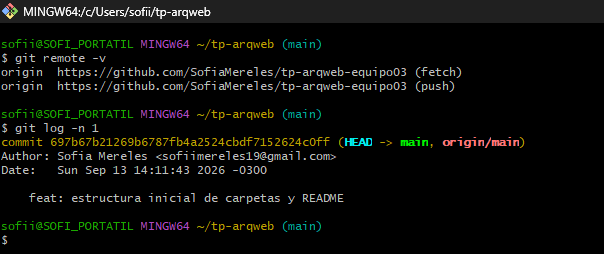
\includegraphics[width=0.85\textwidth]{F1-E1_github_repo.png}
    \caption{F1-E1: Comandos ejecutados en la terminal para la vinculación del repositorio local.}
    \label{fig:F1-E1}
\end{figure}

\begin{figure}[H]
    \centering
    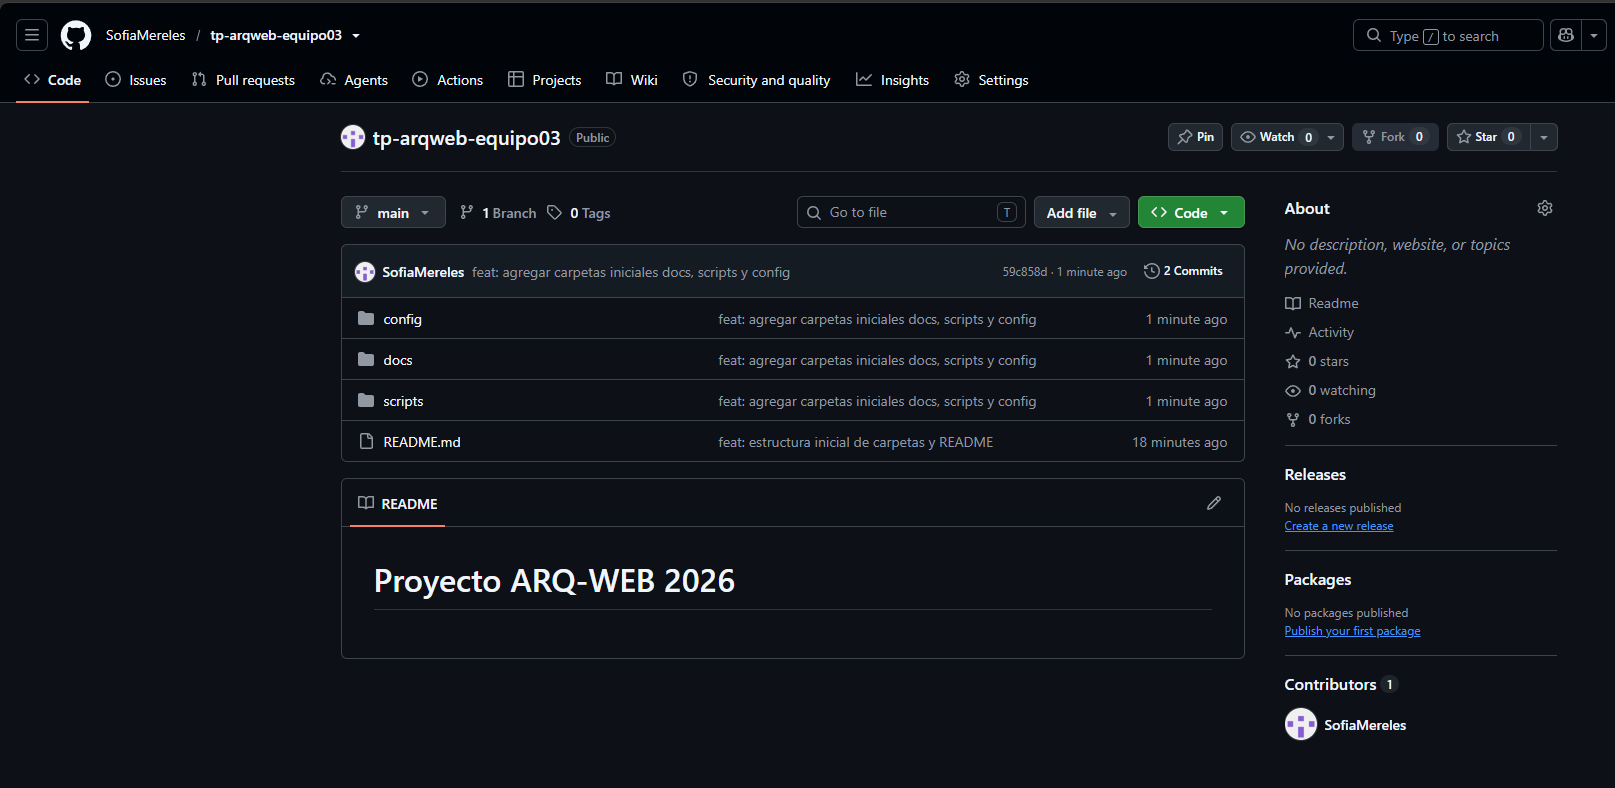
\includegraphics[width=0.85\textwidth]{F1-E2_github_repo.png}
    \caption{F1-E2: Vista web del repositorio público en GitHub con la estructura de directorios.}
    \label{fig:F1-E2}
\end{figure}

\subsection{Especificaciones de la VM}
\begin{itemize}
    \item \textbf{Sistema Operativo:} Ubuntu Server 24.04 LTS
    \item \textbf{Recursos:} 2 vCPU, 4 GB RAM, 20 GB Disco.
    \item \textbf{Modo de Red:} Adaptador Puente (Bridged).
\end{itemize}

\begin{figure}[H]
    \centering
    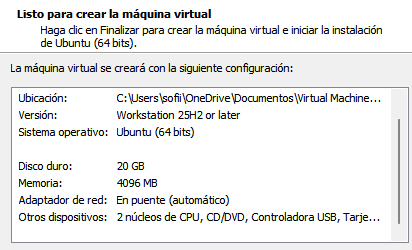
\includegraphics[width=0.85\textwidth]{F1-E3_vmware_hardware.png}
    \caption{F1-E3: Configuración de hardware y red en VMware Workstation.}
    \label{fig:F1-E3}
\end{figure}

\begin{figure}[H]
    \centering
    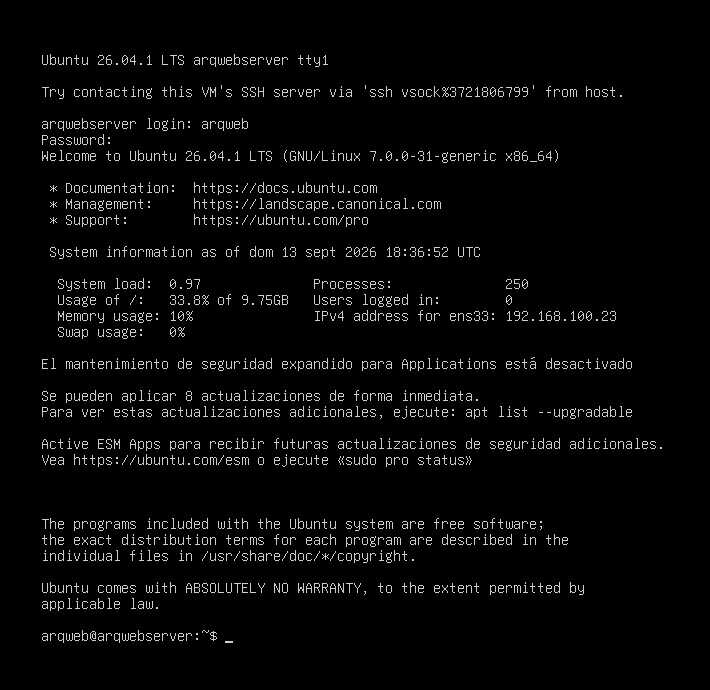
\includegraphics[width=0.85\textwidth]{F1-E4_ubuntu_login.png}
    \caption{F1-E4: Consola de Ubuntu Server operativa con el usuario no-root iniciado.}
    \label{fig:F1-E4}
\end{figure}

\subsection{Línea Base de Red y Direccionamiento}
En la máquina virtual se configuró el adaptador de red en modo puente (\textit{Bridged}), permitiendo obtener la IP \texttt{192.168.100.23/24}.

\begin{figure}[H]
    \centering
    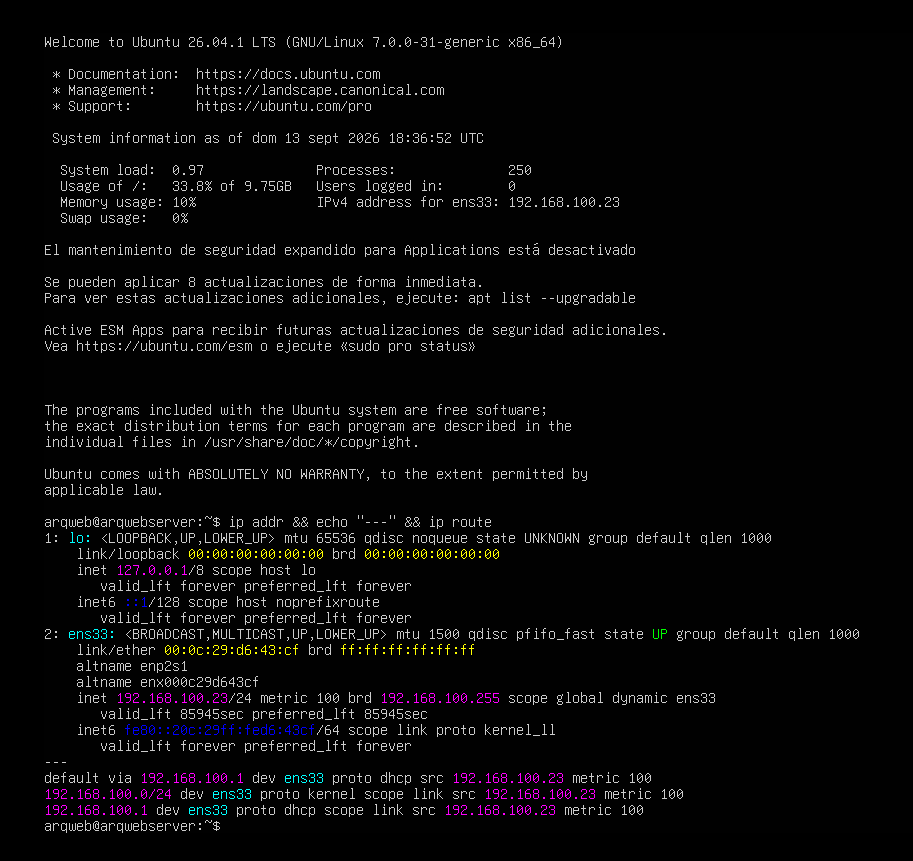
\includegraphics[width=0.85\textwidth]{F1_E5_ip_addr_route.png}
    \caption{F1-E5: Salida del comando \texttt{ip addr} e \texttt{ip route} en Ubuntu Server.}
    \label{fig:F1-E5}
\end{figure}

\begin{figure}[H]
    \centering
    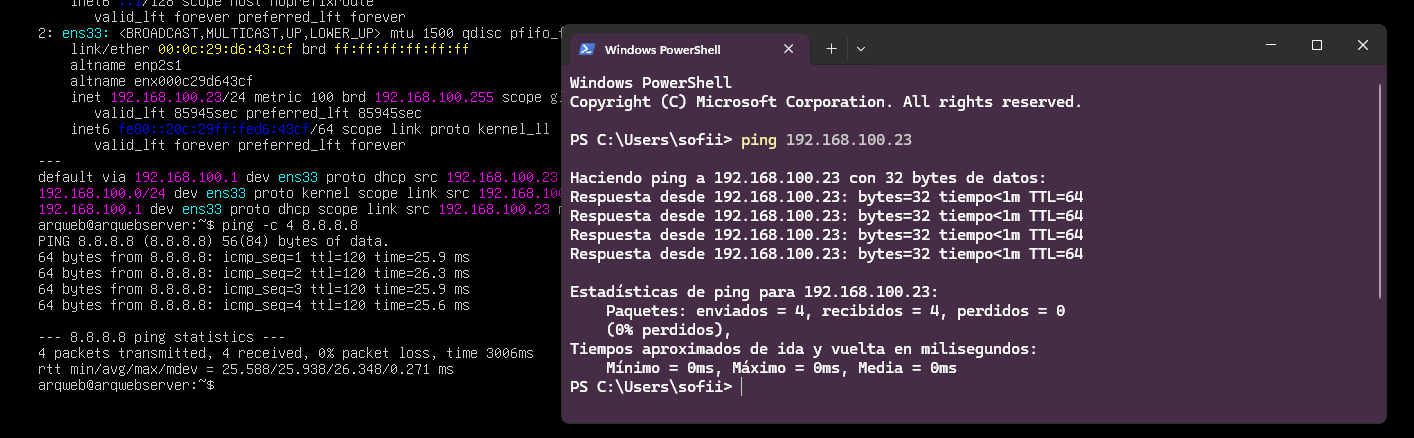
\includegraphics[width=0.85\textwidth]{F1-E6_ping_conectividad.png}
    \caption{F1-E6: Pruebas de conectividad ICMP bidireccional y salida a Internet.}
    \label{fig:F1-E6}
\end{figure}

\begin{figure}[H]
    \centering
    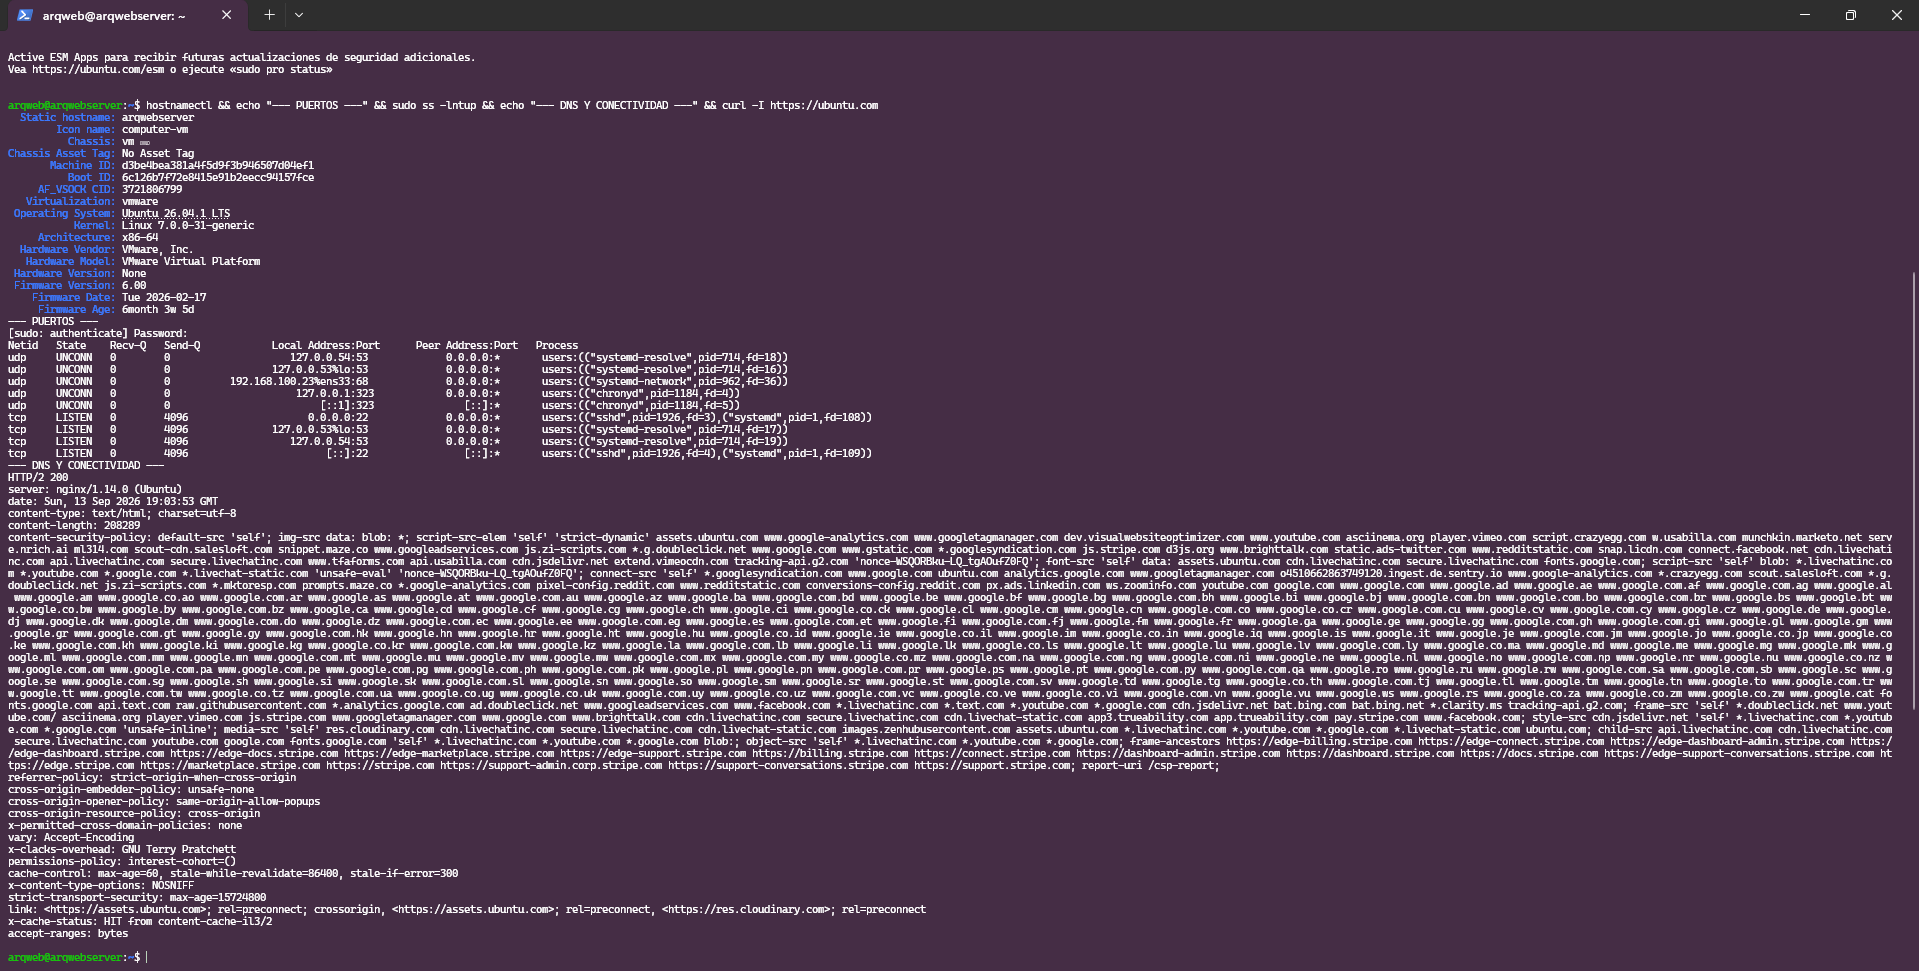
\includegraphics[width=0.85\textwidth]{F1-E7_puertos_dns.png}
    \caption{F1-E7: Verificación del estado del sistema, puerto 22 SSH y resolución DNS.}
    \label{fig:F1-E7}
\end{figure}

\newpage
\section{Despliegue y Configuración de Servicios (Fase 2)}

\subsection{Estado Inicial de los Servicios (F2-E1)}
\begin{figure}[H]
    \centering
    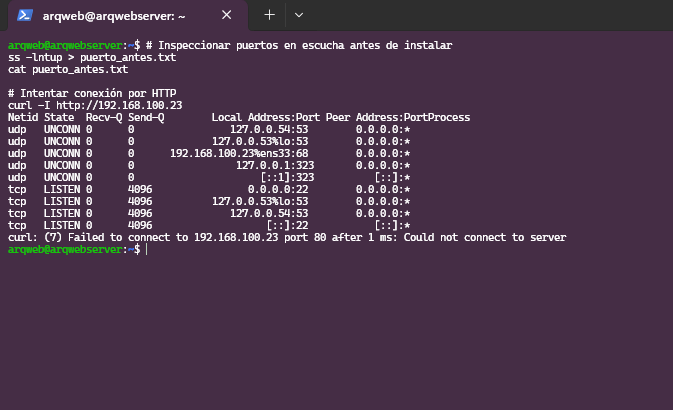
\includegraphics[width=0.92\textwidth]{F2-E1_antes_servicios.png}
    \caption{F2-E1: Verificación del estado de los servicios Nginx, PHP 8.5-FPM y MariaDB.}
    \label{fig:F2-E1}
\end{figure}

\subsection{Verificación de Versiones de Runtime (F2-E2)}
\begin{figure}[H]
    \centering
    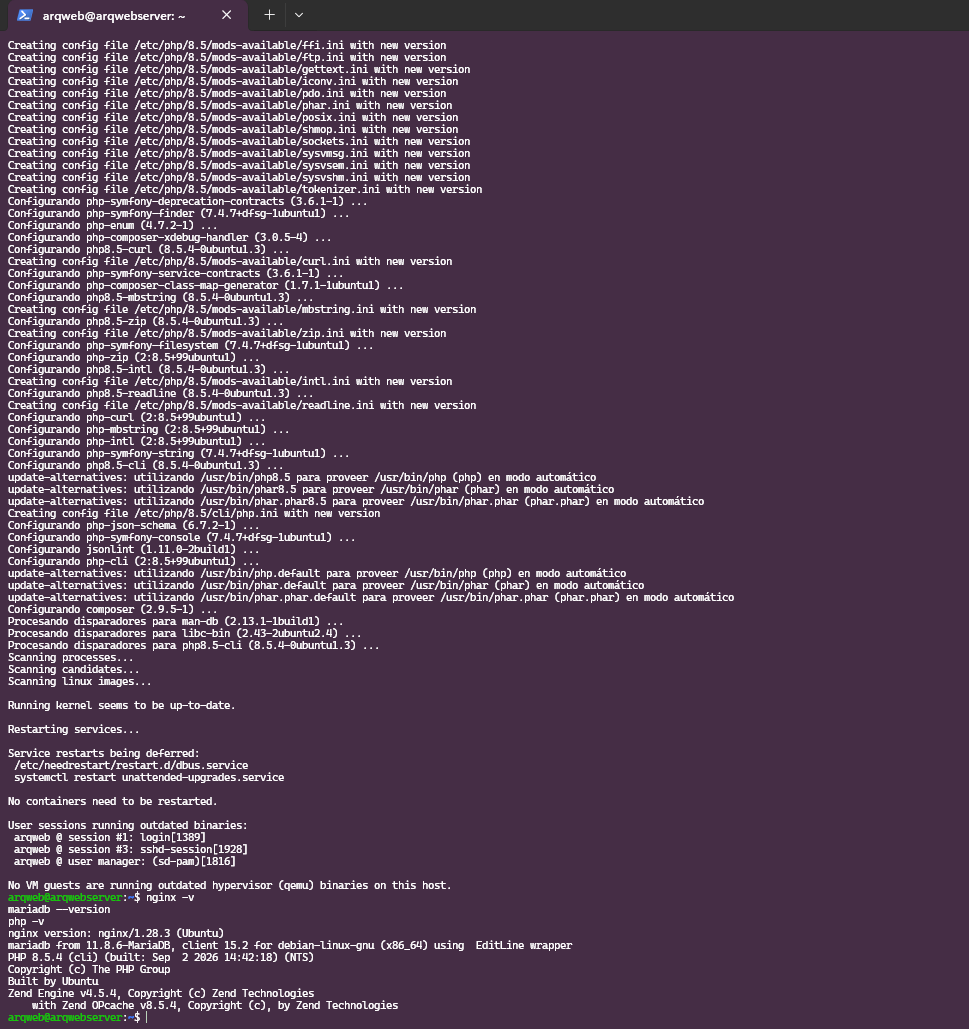
\includegraphics[width=0.75\textwidth]{F2-E2_versiones_runtime.png}
    \caption{F2-E2: Comprobación de versiones activas de Nginx, PHP 8.5 y MariaDB.}
    \label{fig:F2-E2}
\end{figure}

\subsection{Creación y Configuración de la Base de Datos (F2-E3)}
\begin{figure}[H]
    \centering
    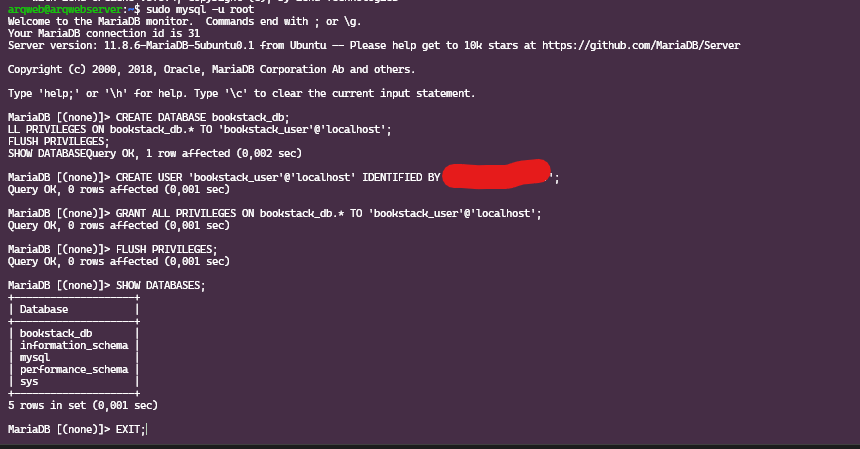
\includegraphics[width=0.88\textwidth]{F2-E3_mariadb_database.png}
    \caption{F2-E3: Sentencias SQL para la creación del esquema y asignación de permisos.}
    \label{fig:F2-E3}
\end{figure}

\subsection{Ejecución de Migraciones de BookStack / Laravel (F2-E4)}
\begin{figure}[H]
    \centering
    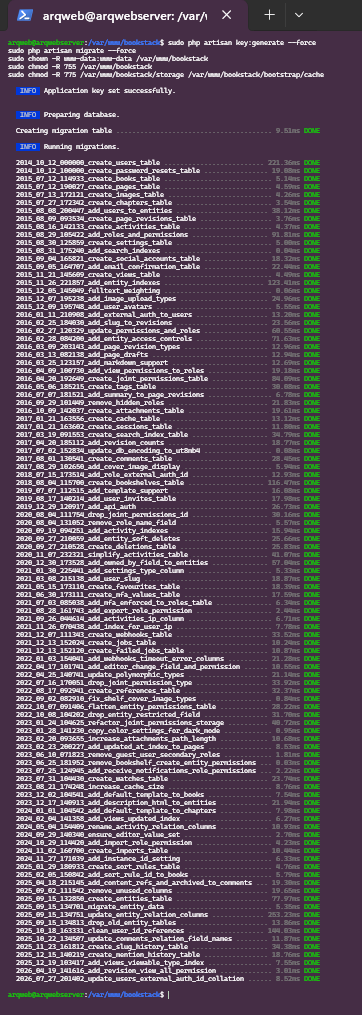
\includegraphics[width=0.55\textwidth]{F2-E4_migracion_laravel.png}
    \caption{F2-E4: Ejecución exitosa de las migraciones de tablas en Laravel para BookStack.}
    \label{fig:F2-E4}
\end{figure}

\subsection{Configuración del Virtual Host y Sintaxis de Nginx (F2-E5)}
\begin{figure}[H]
    \centering
    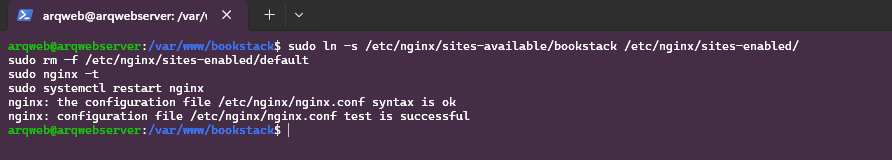
\includegraphics[width=0.90\textwidth]{F2-E5_nginx_sintaxis.png}
    \caption{F2-E5: Verificación de sintaxis exitosa del archivo de configuración de Nginx.}
    \label{fig:F2-E5}
\end{figure}

\subsection{Estado Final de Servicios y Puertos en Escucha (F2-E6)}
\begin{figure}[H]
    \centering
    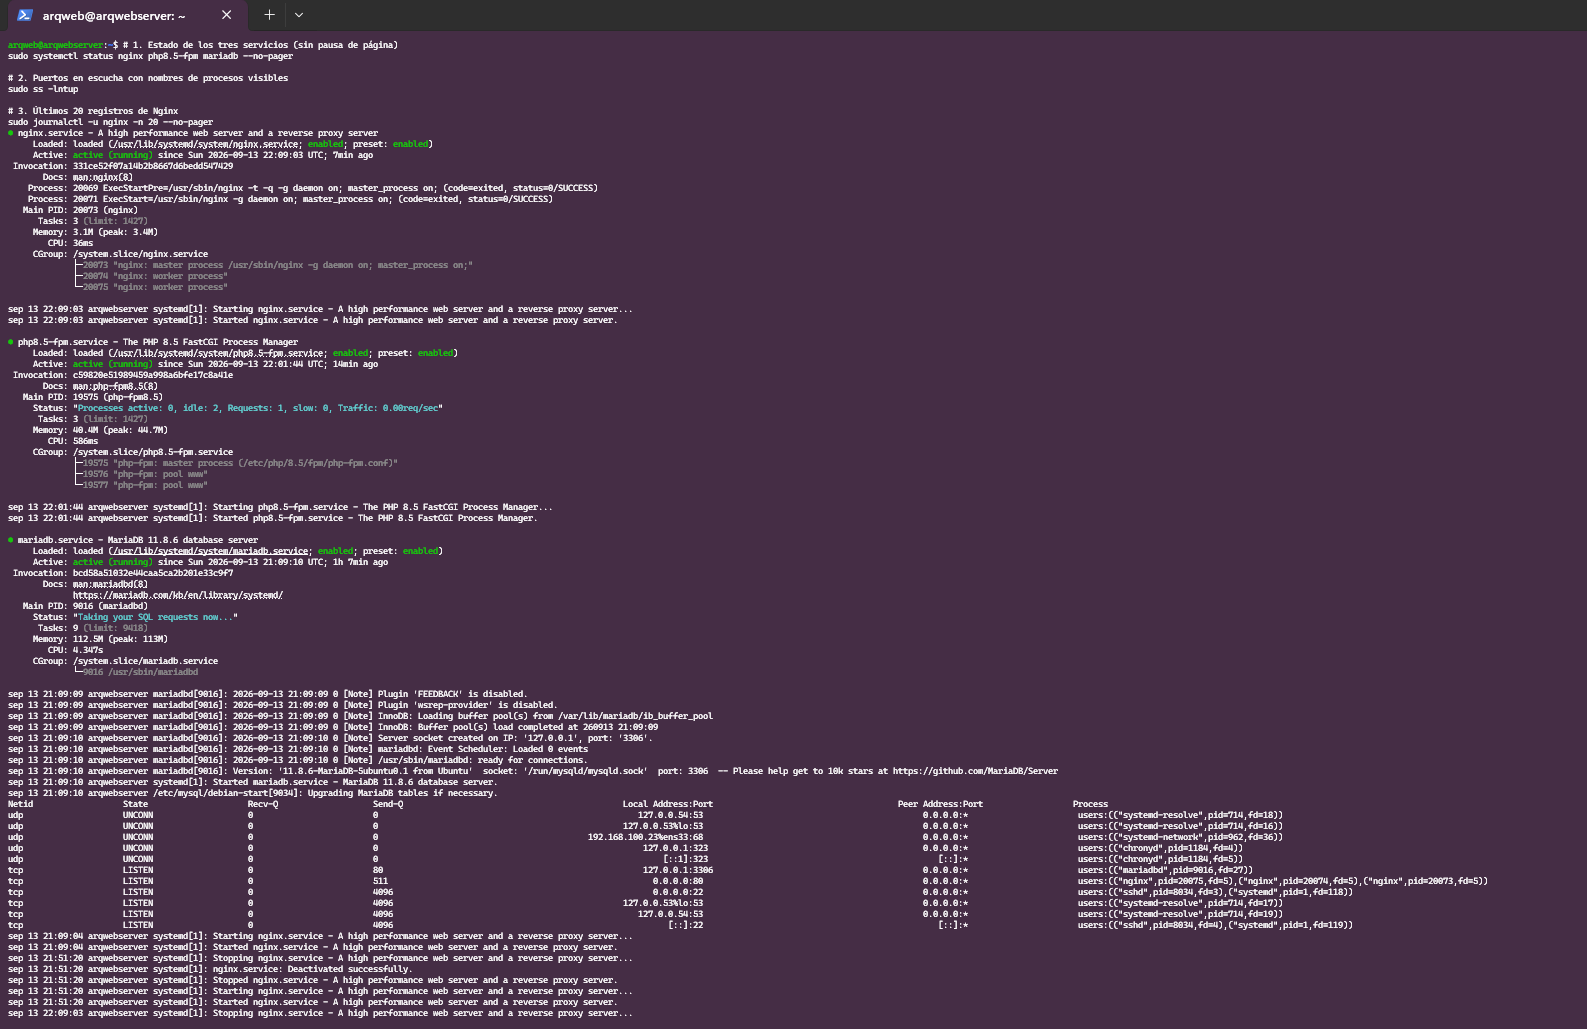
\includegraphics[width=0.95\textwidth]{F2-E6_despues_servicios_puertos.png}
    \caption{F2-E6: Inspección final de servicios activos y sockets en los puertos TCP 80 y TCP 3306.}
    \label{fig:F2-E6}
\end{figure}

\subsection{Pruebas de Conectividad HTTP y Verificación Web Final (F2-E7)}
\begin{figure}[H]
    \centering
    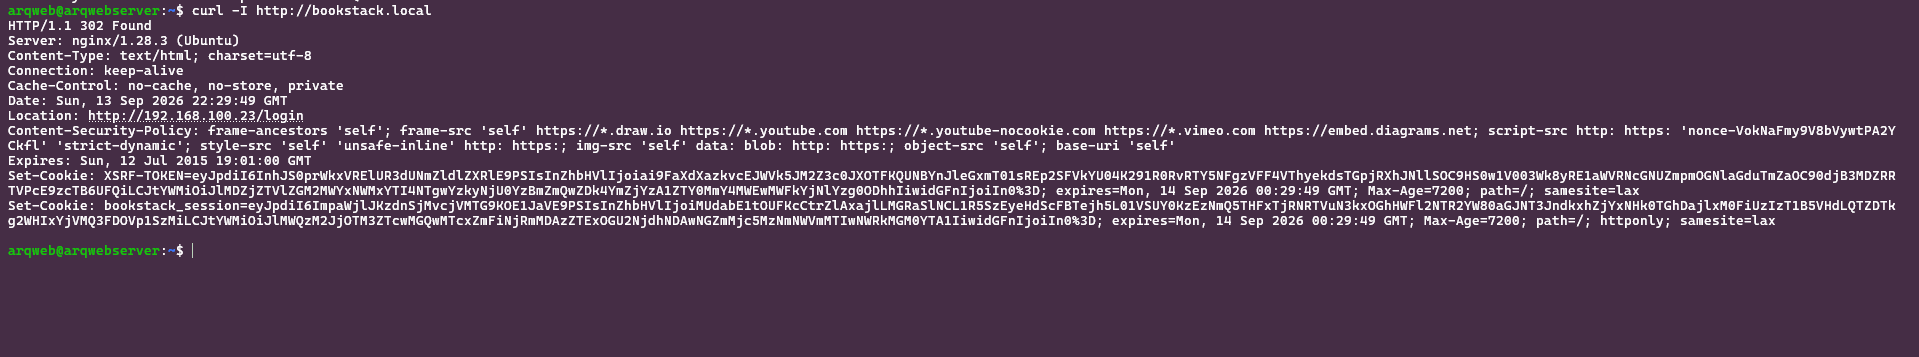
\includegraphics[width=0.85\textwidth]{F2-E7_curl_headers.png}
    \caption{F2-E7a: Respuesta del servidor web mostrando encabezados HTTP mediante \texttt{curl}.}
    \label{fig:F2-E7_curl}
\end{figure}

\begin{figure}[H]
    \centering
    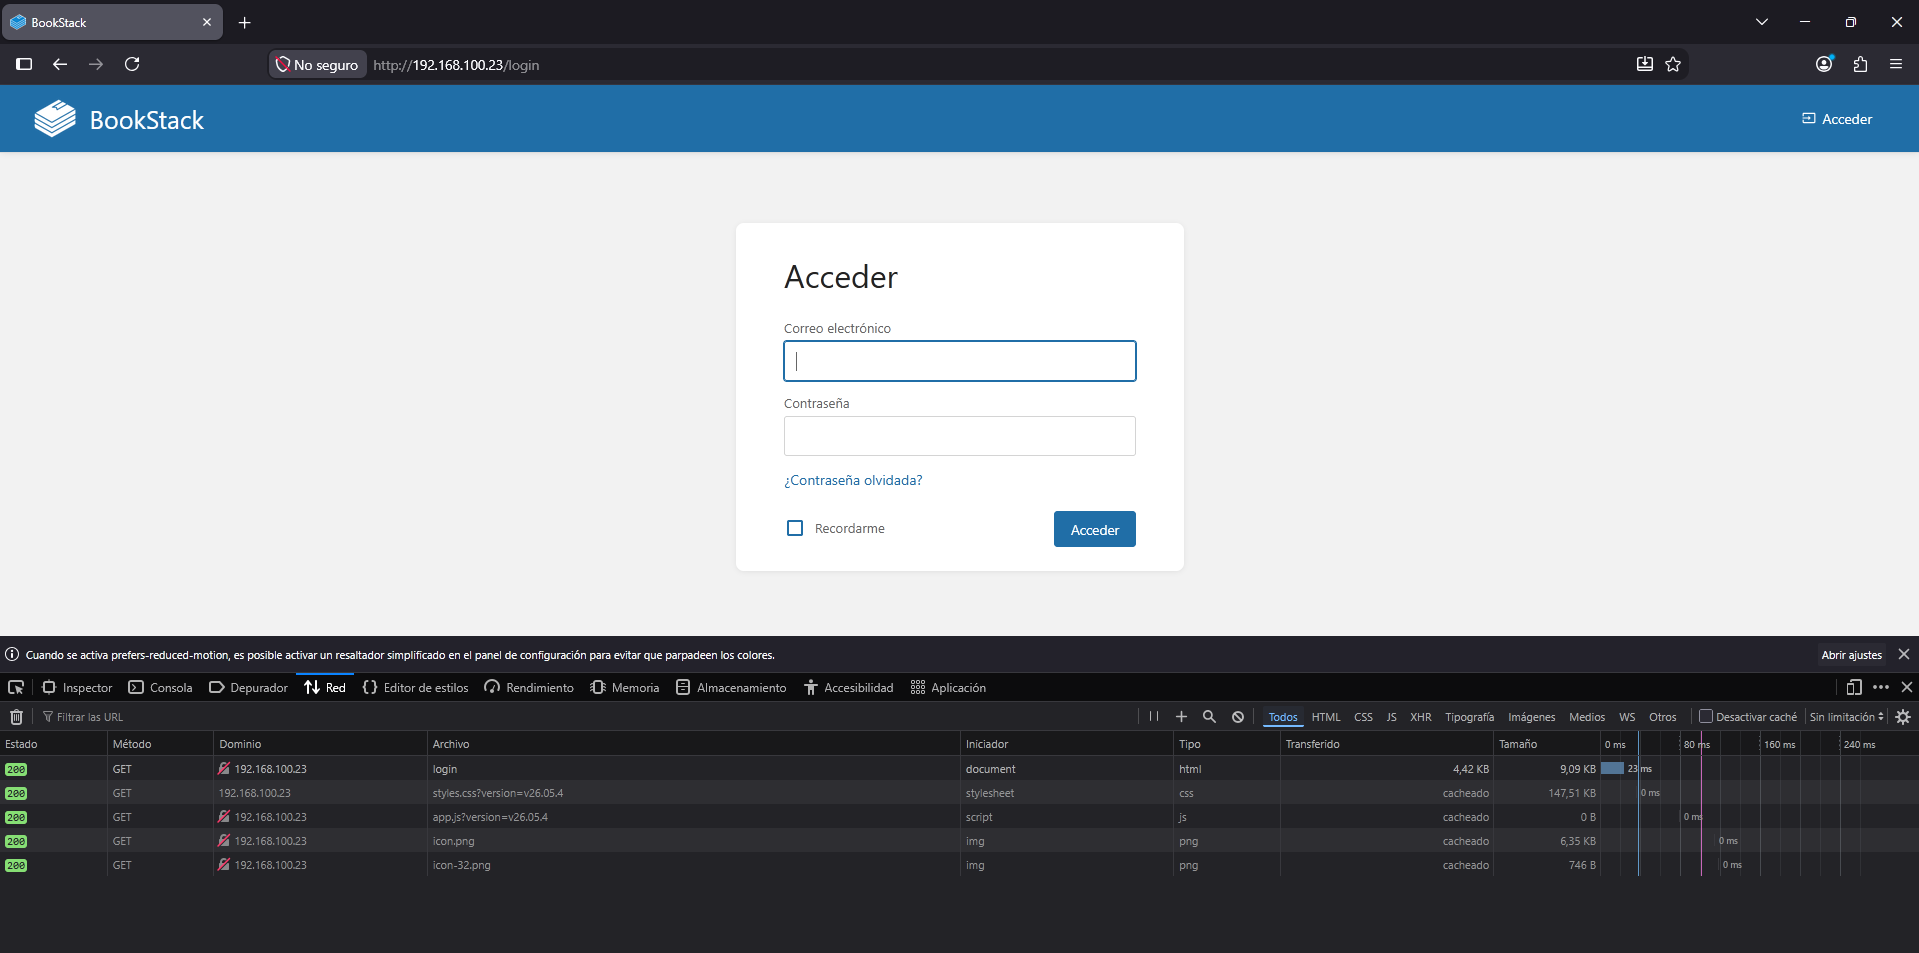
\includegraphics[width=0.95\textwidth]{F2-E7_verificacion_final.png}
    \caption{F2-E7b: Carga completa de la interfaz de login de BookStack y panel DevTools.}
    \label{fig:F2-E7_final}
\end{figure}

\newpage
% =======================================================================
% FASE 3 / ENTREGABLE 3: SEGURIDAD, RENDIMIENTO Y ANÁLISIS DE RED
% =======================================================================
\section{Seguridad, Rendimiento y Análisis de Red (Fase 3)}

En esta sección se detalla la implementación del protocolo HTTPS sobre TLS 1.3, la resolución de nombres local, la optimización de cabeceras/caché, las mediciones de latencia y el análisis de la traza de red capturada.

\subsection{Resolución de Nombres Local y Certificado X.509}

Para simular un entorno de producción con un Fully Qualified Domain Name (FQDN), se asignó el dominio \texttt{bookstack.local} asociándolo a la dirección IP \texttt{192.168.100.23} dentro del archivo de mapeo estático del sistema (\texttt{/etc/hosts}).

\begin{figure}[H]
    \centering
    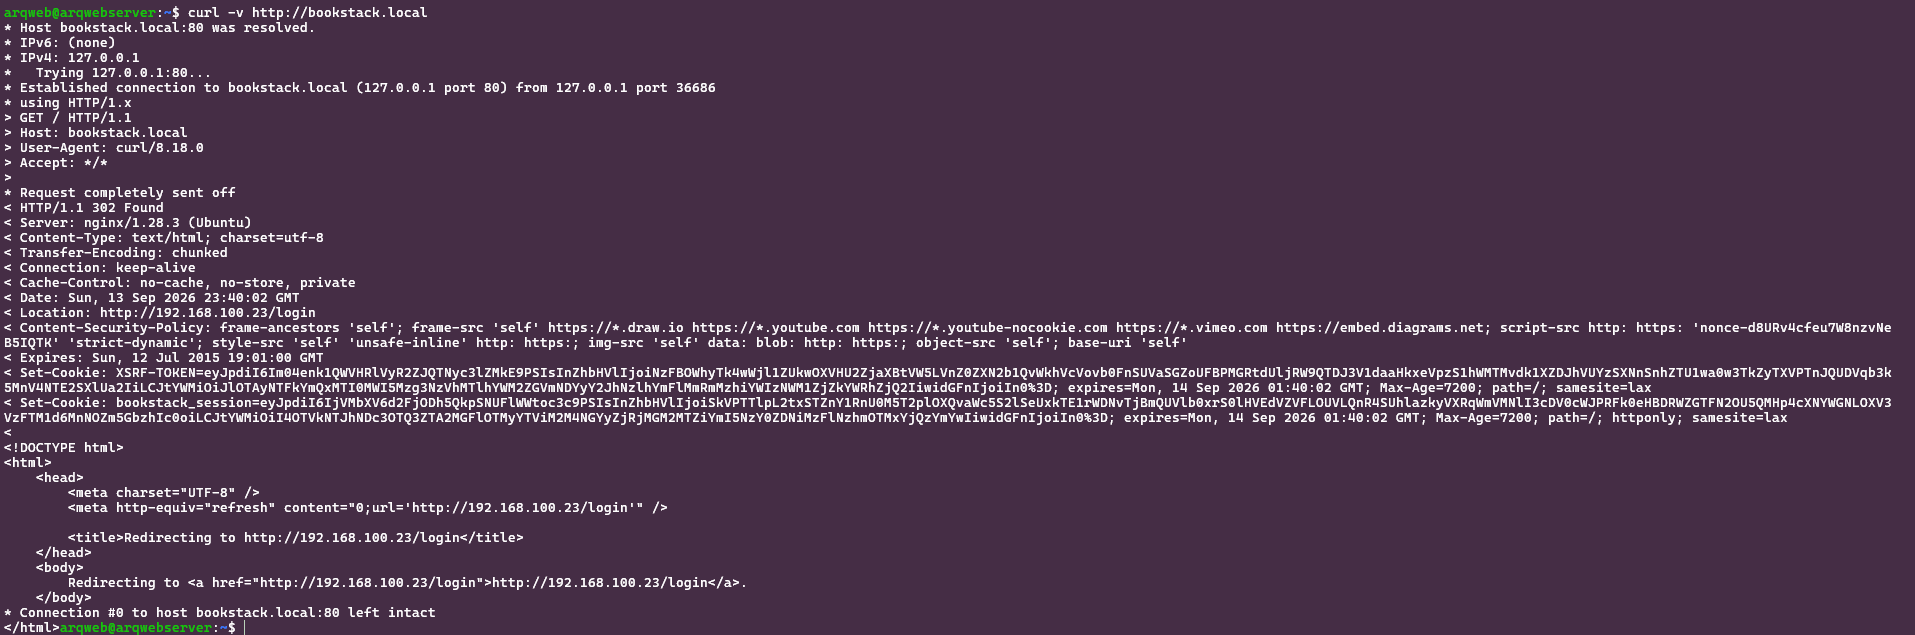
\includegraphics[width=0.85\textwidth]{F2-E1-Resolucion de nombre.png}
    \caption{F3-E1: Configuración de resolución de nombres en \texttt{/etc/hosts} y verificación de conectividad mediante \texttt{ping bookstack.local}.}
    \label{fig:F3-E1}
\end{figure}

En la Figura \ref{fig:F3-E1} (Evidencia F3-E1), se comprueba que el nombre de dominio resuelve correctamente hacia la IP de la máquina virtual con un tiempo de latencia nulo.

A continuación, se generó un certificado digital X.509 autofirmado mediante el kit de herramientas OpenSSL, especificando una extensión Subject Alternative Name (SAN) para garantizar la compatibilidad con navegadores modernos:

\begin{figure}[H]
    \centering
    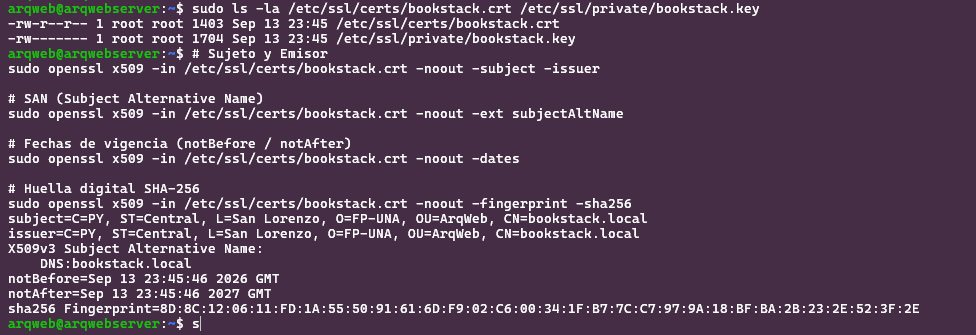
\includegraphics[width=0.92\textwidth]{F2-E2-Certificado-local.png}
    \caption{F3-E2: Inspección del certificado X.509 emitido con OpenSSL (\texttt{CN=bookstack.local}, algoritmo RSA 2048 bits y huella digital SHA-256).}
    \label{fig:F3-E2}
\end{figure}

Como evidencia la Figura \ref{fig:F3-E2} (Evidencia F3-E2), la inspección del archivo \texttt{/etc/ssl/certs/bookstack.crt} confirma la validez del certificado, la vigencia de un año, el algoritmo de firma \texttt{sha256WithRSAEncryption} y la huella digital correspondiente.

\paragraph{Análisis de la Cadena de Confianza y Advertencias del Navegador:}
Al acceder a un sitio configurado con un certificado autofirmado, el navegador emite una advertencia de seguridad (\textit{"La conexión no es privada"}). Esto ocurre porque la Autoridad Certificadora (CA) emisora es la misma entidad que el sujeto (\texttt{Issuer = Subject}), por lo que la CA no se encuentra dentro del almacén de confianza preinstalado en el sistema operativo cliente (\textit{Root CA Store}). Para un entorno de producción real, este paso se sustituye por la emisión de un certificado validado por una CA pública (ej. Let's Encrypt).

\subsection{Configuración de la Aplicación y Server Block en Nginx}

Para garantizar la coherencia de la aplicación Laravel con la capa de transporte segura, se actualizó el archivo de entorno global \texttt{.env} de BookStack ajustando la variable de URL base:

\begin{figure}[H]
    \centering
    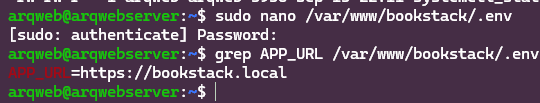
\includegraphics[width=0.85\textwidth]{F3-E3-VERIFICACION APP_URL.png}
    \caption{F3-E3: Verificación de la variable de entorno \texttt{APP\_URL=https://bookstack.local} en el archivo \texttt{.env}.}
    \label{fig:F3-E3}
\end{figure}

En la Figura \ref{fig:F3-E3} (Evidencia F3-E3), el comando \texttt{grep} confirma que los recursos estáticos, enlaces absolutos y cookies de sesión sean generados bajo el esquema seguro HTTPS.

Posteriormente, se reestructuró el archivo de bloque de servidor de Nginx (\texttt{/etc/nginx/sites-available/bookstack}) dividiéndolo en dos bloques \texttt{server}:
\begin{enumerate}
    \item \textbf{Bloque HTTP (Puerto 80):} Captura todas las peticiones inseguras e inyecta una redirección permanente \texttt{HTTP 301 Moved Permanently} hacia \texttt{https://bookstack.local\$request\_uri}.
    \item \textbf{Bloque HTTPS (Puerto 443):} Configura la escucha en modo SSL (\texttt{listen 443 ssl;}), enlaza la clave privada y certificado, limita los protocolos a \textbf{TLS 1.2} y \textbf{TLS 1.3}, y deriva la ejecución PHP al socket Unix de PHP-FPM.
\end{enumerate}

\begin{figure}[H]
    \centering
    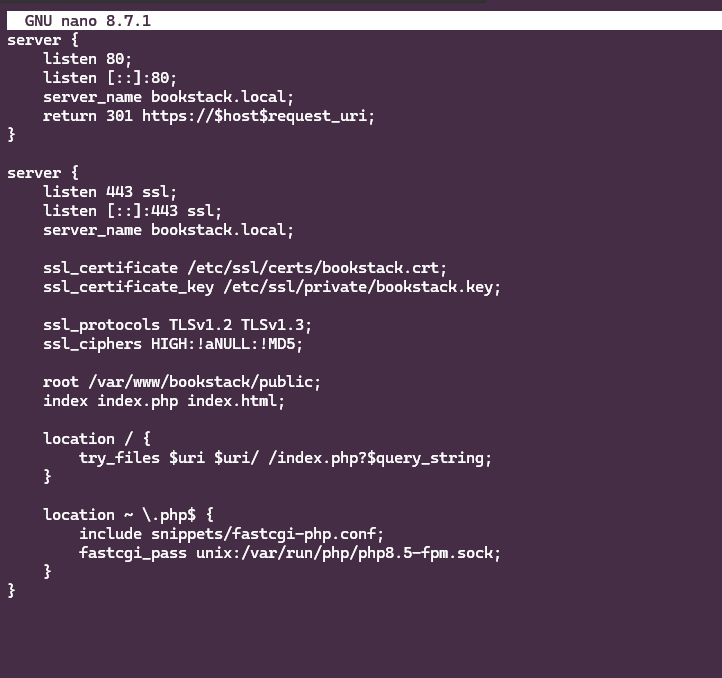
\includegraphics[width=0.75\textwidth]{F3-E4-Virtual Host de Nginx.png}
    \caption{F3-E4: Edición del Server Block en Nginx habilitando SSL/TLS 1.3 en el puerto 443 y redirección HTTP 301.}
    \label{fig:F3-E4}
\end{figure}

La Figura \ref{fig:F3-E4} (Evidencia F3-E4) muestra las directivas aplicadas en la configuración de Nginx.

\subsection{Evaluación Experimental de Rendimiento HTTPS}

Se ejecutó un script en Bash realizando 10 iteraciones consecutivas mediante el comando \texttt{curl -w} para descomponer los tiempos de conexión en cada fase del modelo de red:

\begin{figure}[H]
    \centering
    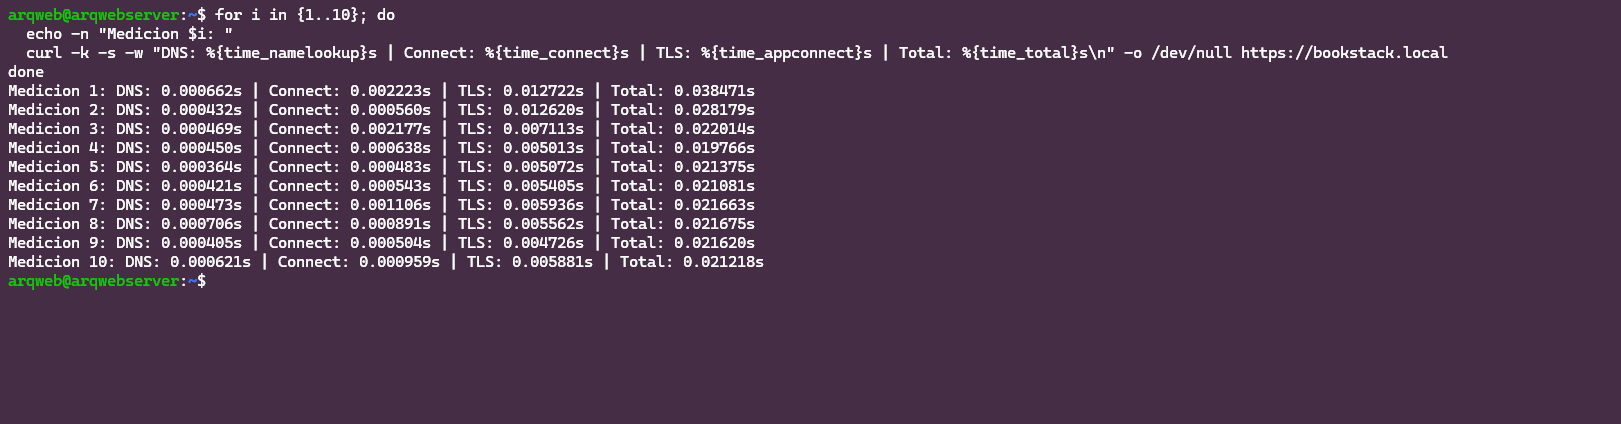
\includegraphics[width=0.95\textwidth]{F2-E5-Medición de rendimiento.png}
    \caption{F3-E5: Ejecución secuencial de 10 mediciones de rendimiento con \texttt{curl} sobre la conexión HTTPS.}
    \label{fig:F3-E5}
\end{figure}

Como muestra la Figura \ref{fig:F3-E5} (Evidencia F3-E5), se registraron los métricos consolidados en la Tabla \ref{tab:rendimiento}.

\begin{table}[h!]
\centering
\small
\begin{tabular}{|c|c|c|c|c|}
\hline
\textbf{Iteración} & \textbf{DNS Lookup (s)} & \textbf{TCP Connect (s)} & \textbf{TLS Handshake (s)} & \textbf{Tiempo Total (s)} \\ \hline
1 & 0.000662 & 0.002223 & 0.012722 & 0.038471 \\ \hline
2 & 0.000432 & 0.000560 & 0.012620 & 0.028179 \\ \hline
3 & 0.000469 & 0.002177 & 0.007113 & 0.022014 \\ \hline
4 & 0.000450 & 0.000638 & 0.005013 & 0.019766 \\ \hline
5 & 0.000364 & 0.000483 & 0.005072 & 0.021375 \\ \hline
6 & 0.000421 & 0.000543 & 0.005405 & 0.021081 \\ \hline
7 & 0.000473 & 0.001106 & 0.005936 & 0.021663 \\ \hline
8 & 0.000706 & 0.000891 & 0.005562 & 0.021675 \\ \hline
9 & 0.000405 & 0.000504 & 0.004726 & 0.021620 \\ \hline
10 & 0.000621 & 0.000959 & 0.005881 & 0.021218 \\ \hline
\textbf{Promedio} & \textbf{0.000500s (0.50 ms)} & \textbf{0.001008s (1.01 ms)} & \textbf{0.007005s (7.00 ms)} & \textbf{0.023706s (23.71 ms)} \\ \hline
\end{tabular}
\caption{Desglose de tiempos de respuesta en la negociación HTTPS (10 iteraciones).}
\label{tab:rendimiento}
\end{table}

\paragraph{Interpretación Técnica de los Resultados:}
\begin{itemize}
    \item \textbf{Efecto Calentamiento (\textit{Warm-up}):} La primera medición registró un tiempo total de 38.4 ms debido a la lectura inicial en disco de los certificados y la inicialización de procesos en el worker de PHP-FPM.
    \item \textbf{Optimización por Reuso de Sesión TLS:} A partir de la iteración 4, el tiempo de negociación TLS disminuyó de 12.7 ms a ~5.0 ms. Esto se debe al uso de \textit{TLS Session Tickets} en TLS 1.3, eliminando un viaje de ida y vuelta (\textit{RTT}) en reconexiones.
    \item \textbf{Estabilidad:} El sistema demostró un tiempo de procesamiento promedio de \textbf{23.71 ms}, manteniendo una desviación estándar mínima en el entorno virtualizado.
\end{itemize}

\subsection{Inspección de Cabeceras HTTP, Compresión y Caché}

Se analizó la respuesta del servidor mediante \texttt{curl -I} enviando la cabecera \texttt{Accept-Encoding: gzip} para auditar las políticas de caché y compresión de datos:

\begin{figure}[H]
    \centering
    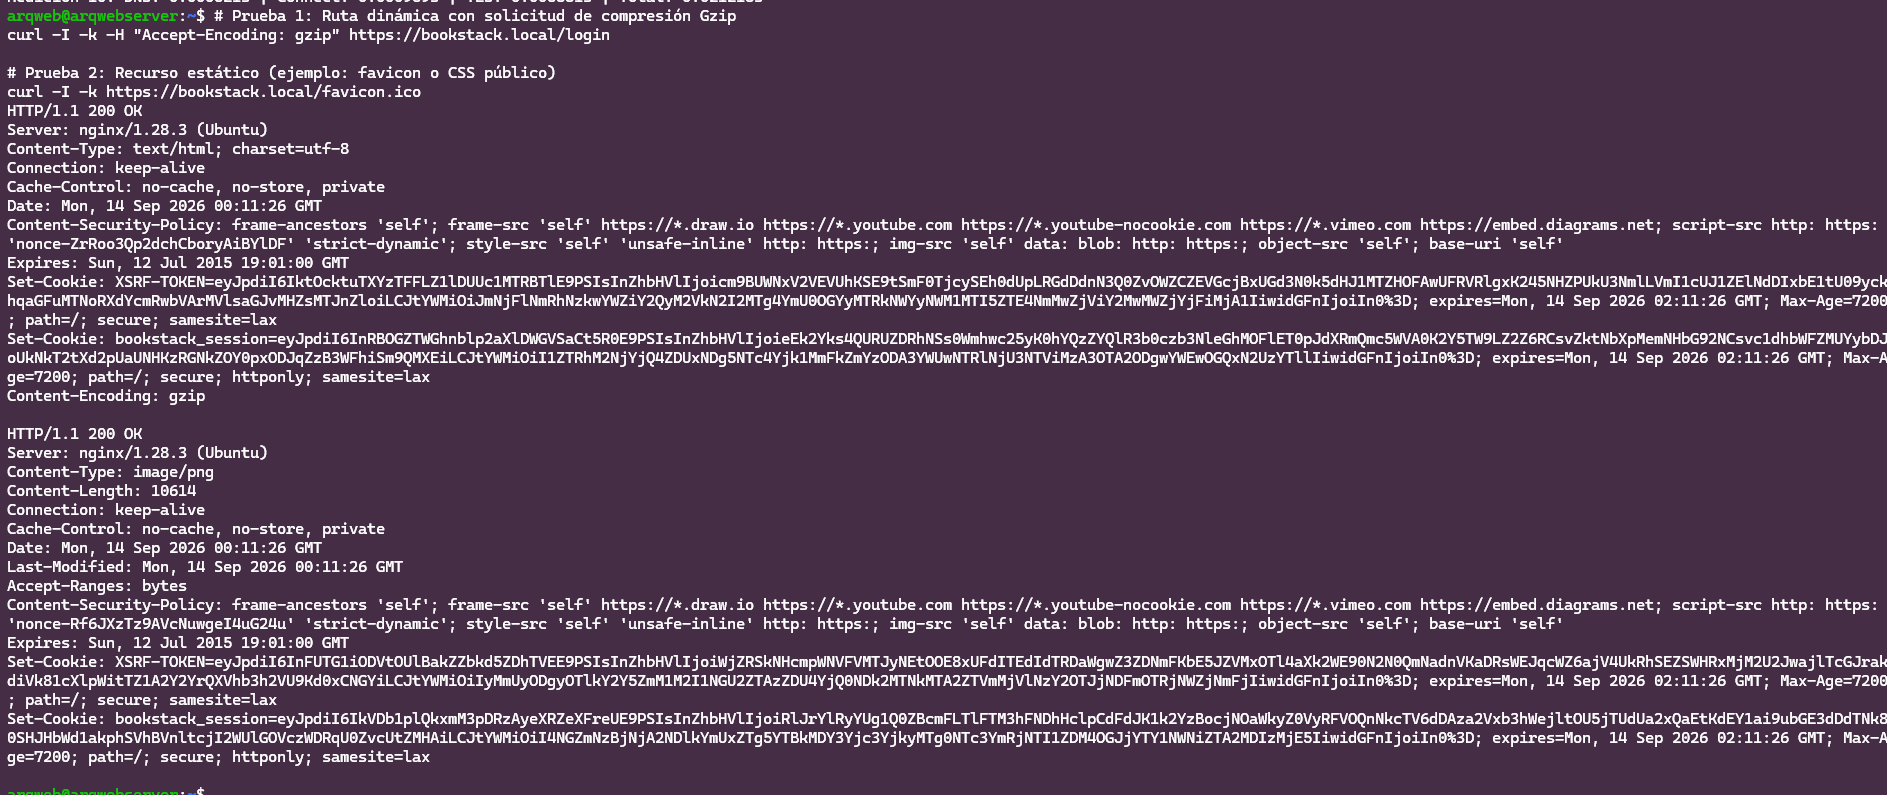
\includegraphics[width=0.95\textwidth]{F3-E6-evidencia_compresion_y_cache.png}
    \caption{F3-E6: Verificación de cabeceras HTTP de respuesta: \texttt{Content-Encoding: gzip}, \texttt{Cache-Control}, cookies \texttt{secure} y marca \texttt{Last-Modified}.}
    \label{fig:F3-E6}
\end{figure}

Como evidencia la Figura \ref{fig:F3-E6} (Evidencia F3-E6), se identifican los siguientes comportamientos:
\begin{itemize}
    \item \textbf{Compresión Dinámica:} La presencia de \texttt{Content-Encoding: gzip} confirma que Nginx comprime el cuerpo HTML antes de la transmisión, reduciendo el consumo de ancho de banda.
    \item \textbf{Caché en Rutas Dinámicas:} La cabecera \texttt{Cache-Control: no-cache, no-store, private} previene que páginas transaccionales con tokens CSRF o cookies de sesión sean almacenadas en proxies intermedios.
    \item \textbf{Atributos de Cookies Seguras:} Las cookies \texttt{XSRF-TOKEN} y \texttt{bookstack\_session} incluyen las directivas \texttt{secure} y \texttt{httponly}, garantizando que solo viajen sobre HTTPS y no sean accesibles mediante código JavaScript de cliente.
    \item \textbf{Validación Condicional 304 (Not Modified):} Para recursos estáticos, Nginx entrega la cabecera \texttt{Last-Modified}. Ante peticiones subsecuentes del cliente con \texttt{If-Modified-Since}, el servidor responde con el código \texttt{HTTP 304 Not Modified}, omitiendo el envío del archivo y ahorrando recursos de red.
\end{itemize}

\subsection{Comparativa de Arquitectura: Acceso Directo al Backend vs. Proxy Inverso}

A continuación se analizan las diferencias operativas entre exponer directamente el motor de ejecución o utilizar Nginx como Proxy Inverso:

\begin{table}[h!]
\centering
\small
\begin{tabular}{|p{3.5cm}|p{5.5cm}|p{5.5cm}|}
\hline
\textbf{Criterio} & \textbf{Acceso Directo (PHP-FPM)} & \textbf{Proxy Inverso (Nginx)} \\ \hline
\textbf{Protocolo Soportado} & Exclusivamente protocolo binario \textbf{FastCGI}. No habla HTTP de forma nativa. & \textbf{HTTP/1.1, HTTP/2, HTTPS (TLS 1.2/1.3)}. Traduce HTTP a FastCGI. \\ \hline
\textbf{Terminación TLS} & Sin soporte nativo de cifrado X.509/TLS. Tráfico transmitido en texto plano. & Gestiona el certificado SSL/TLS, descifrado y suites de cifrado simétrico. \\ \hline
\textbf{Archivos Estáticos} & Ineficiente. Carga el intérprete PHP para entregar imágenes, CSS o JS. & Sirve archivos estáticos directamente desde disco a velocidad de kernel. \\ \hline
\textbf{Seguridad / Aislamiento} & Exponer el socket TCP (ej. 9000) abre vectores de Ejecución Remota de Código (RCE). & Aísla el backend, sanitiza encabezados y limita el tamaño de payload. \\ \hline
\end{tabular}
\caption{Comparativa entre acceso directo al backend PHP-FPM y proxy inverso Nginx.}
\label{tab:comparativa_proxy}
\end{table}

\textbf{Conclusión de Arquitectura:} No es seguro ni técnicamente viable exponer directamente PHP-FPM a la red. Nginx actúa como una capa indispensable de terminación SSL, optimización de caché, entrega de recursos estáticos y protección del motor de la aplicación.

\subsection{Captura y Análisis de Tráfico de Red con \texttt{tcpdump}}

Se registró el tráfico de red mediante la herramienta CLI \texttt{tcpdump} almacenando la transacción en el archivo \texttt{~/transaccion\_tp3.pcap}. Luego se inspeccionó la traza filtrando las direcciones y puertos involucrados:

\begin{figure}[H]
    \centering
    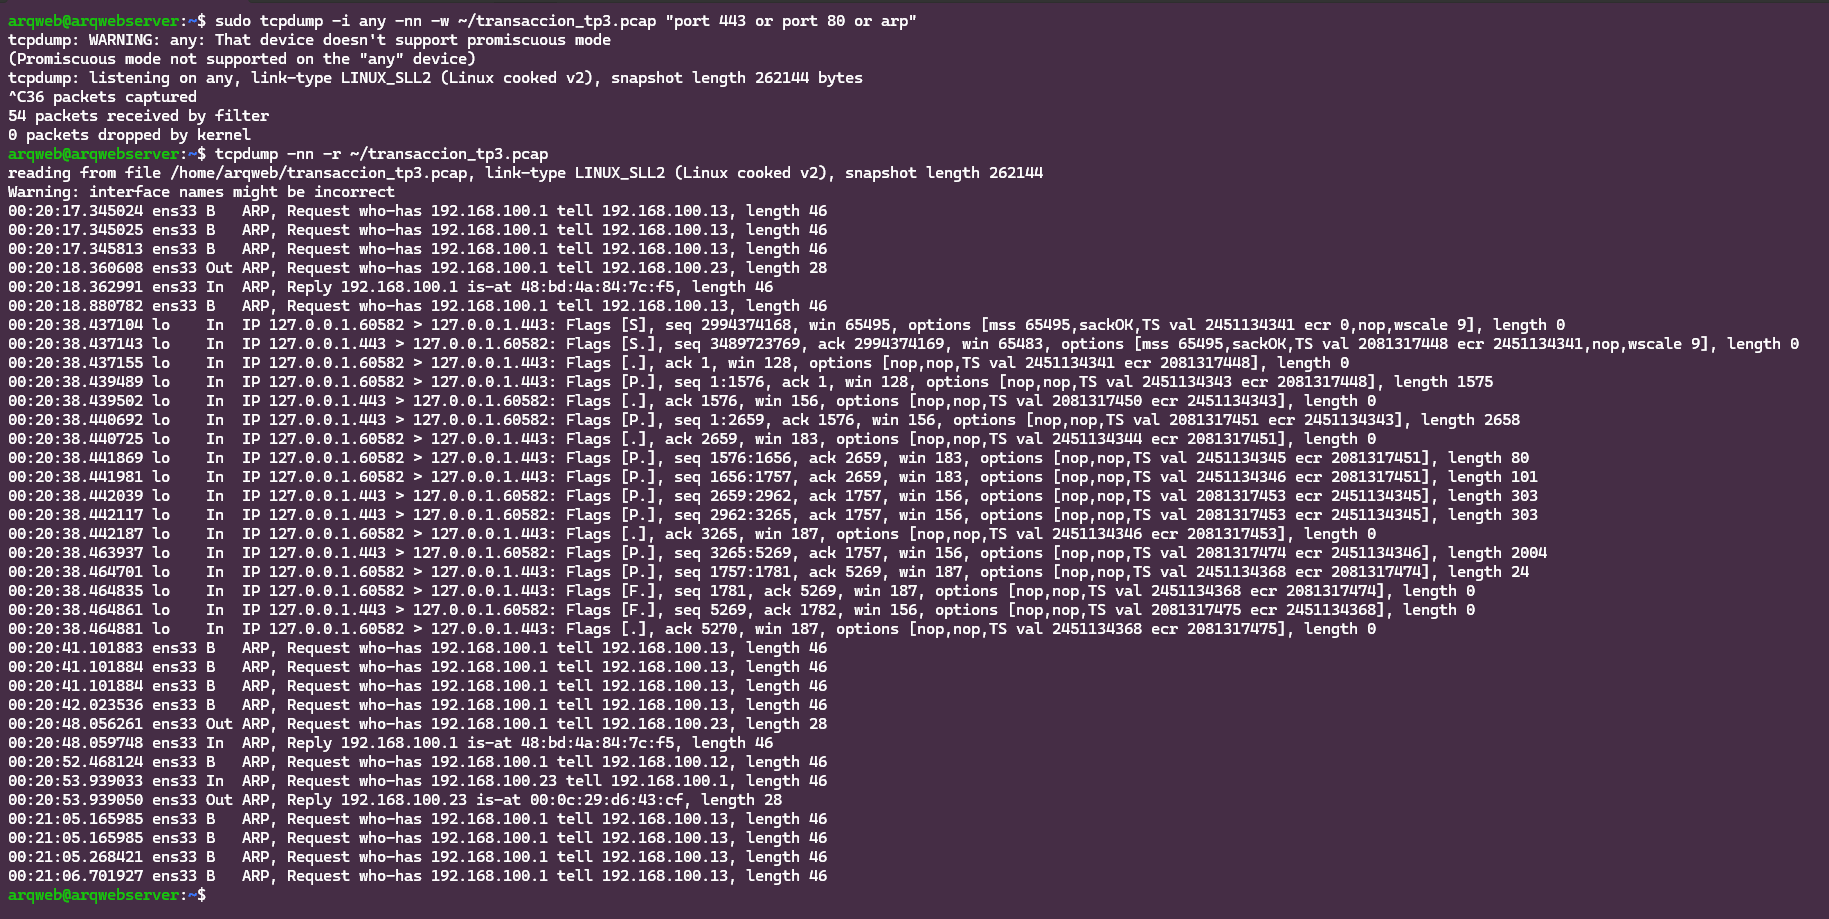
\includegraphics[width=0.98\textwidth]{F2-E7-evidencia_trafico_tcp_tls_arp.png}
    \caption{F3-E7: Traza de paquetes capturada con \texttt{tcpdump} detallando la secuencia ARP, 3-Way Handshake TCP, TLS 1.3 y tramas de datos encriptados.}
    \label{fig:F3-E7}
\end{figure}

En la Figura \ref{fig:F3-E7} (Evidencia F3-E7) se aprecia el desglose cronológico de las tramas, analizado en detalle en la Tabla \ref{tab:analisis_tcpdump}.

\begin{table}[h!]
\centering
\small
\begin{tabular}{|c|c|p{3.2cm}|p{5.8cm}|}
\hline
\textbf{Marca de Tiempo} & \textbf{Capa / Protocolo} & \textbf{Banderas / Tipo} & \textbf{Descripción Técnica de la Transacción} \\ \hline
\texttt{00:20:18.360} & Capa 2 / ARP & \texttt{Request / Reply} & Consulta \textit{broadcast} para obtener la dirección MAC física del Gateway (\texttt{192.168.100.1}). \\ \hline
\texttt{00:20:38.437} & Capa 4 / TCP & \texttt{Flags [S]} (SYN) & \textbf{Handshake (1/3):} Cliente (\texttt{127.0.0.1:60582}) solicita conexión al puerto HTTPS (\texttt{443}). \\ \hline
\texttt{00:20:38.437} & Capa 4 / TCP & \texttt{Flags [S.]} (SYN-ACK) & \textbf{Handshake (2/3):} Nginx confirma la disponibilidad para la apertura del socket. \\ \hline
\texttt{00:20:38.437} & Capa 4 / TCP & \texttt{Flags [.]} (ACK) & \textbf{Handshake (3/3):} Establecimiento completo del canal de transporte TCP. \\ \hline
\texttt{00:20:38.439} & Capa 6 / TLS 1.3 & \texttt{Flags [P.]}, 1575 B & \textbf{Client Hello:} Envío de algoritmos de cifrado y extensión SNI (\texttt{bookstack.local}). \\ \hline
\texttt{00:20:38.440} & Capa 6 / TLS 1.3 & \texttt{Flags [P.]}, 2658 B & \textbf{Server Hello:} Nginx envía su certificado X.509 y establece el cifrado simétrico. \\ \hline
\texttt{00:20:38.441} & Capa 7 / HTTPS & \texttt{Application Data} & Intercambio de peticiones y respuestas HTTP/1.1 cifradas e ilegibles en texto plano. \\ \hline
\texttt{00:20:38.464} & Capa 4 / TCP & \texttt{Flags [F.]} (FIN-ACK) & Intercambio de banderas FIN para el cierre ordenado de la sesión TCP. \\ \hline
\end{tabular}
\caption{Análisis detallado de la captura de paquetes de red (\texttt{transaccion\_tp3.pcap}).}
\label{tab:analisis_tcpdump}
\end{table}

\paragraph{Consideración sobre el Tráfico DNS en la Traza:}
En la captura no se registran paquetes de consulta DNS en el puerto 53/UDP. Esto justifica formalmente que la resolución del FQDN \texttt{bookstack.local} fue resuelta a nivel de kernel mediante la tabla del archivo local \texttt{/etc/hosts}, omitiendo el envío de peticiones a servidores DNS externos.

\subsection{Verificación Final desde Navegador con DevTools (F3-E8)}

Como paso de validación final, se accedió a la plataforma desde el navegador web habilitando el panel de inspección DevTools en la pestaña \textbf{Network}:

\begin{figure}[H]
    \centering
    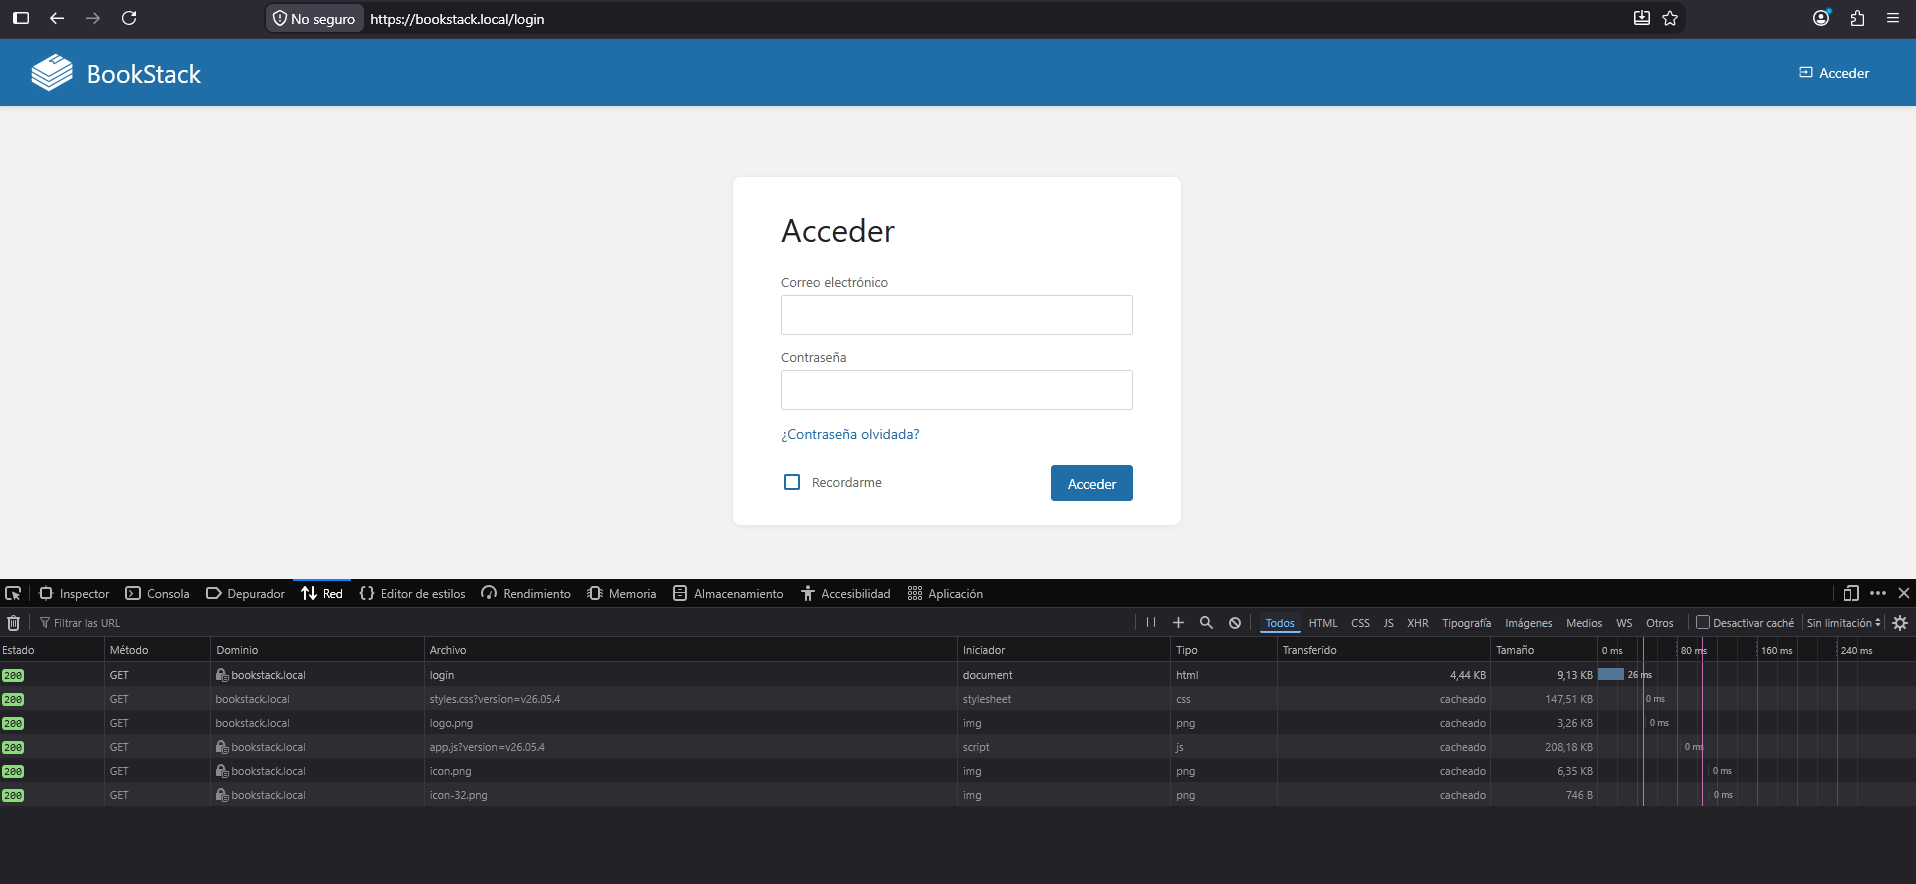
\includegraphics[width=0.95\textwidth]{F3-E8-validacion_network.png}
    \caption{F3-E8: Carga final del formulario de inicio de sesión de BookStack en el navegador web sobre HTTPS (\texttt{bookstack.local}) con el panel DevTools de red activo.}
    \label{fig:F3-E8}
\end{figure}

Como evidencia la Figura \ref{fig:F3-E8} (Evidencia F3-E8), el navegador confirma la conexión cifrada bajo HTTPS, la descarga exitosa de los recursos estáticos (CSS, JS) y la correcta gestión de la sesión del usuario.

\newpage
% =======================================================================
% FASE 4 / ENTREGABLE 4: RESILIENCIA, SEGURIDAD AVANZADA Y DEFENSA
% =======================================================================
\section{Resiliencia, Seguridad Avanzada, Cierre y Defensa (Fase 4)}

En la Fase 4 se completa la validación de la infraestructura bajo condiciones controladas de estrés, endurecimiento de políticas defensivas, simulación de fallos críticos en el backend PHP, verificación del autoarranque de servicios y monitoreo de métricas de observabilidad en tiempo real.

\subsection{Verificación de Firewall y Superficie Expuesta}
Se aplicó el principio de mínimo privilegio sobre el firewall \texttt{ufw}, denegando todo tráfico de red entrante excepto las excepciones explícitamente autorizadas para el funcionamiento del servicio web y la administración remota.

\begin{figure}[H]
    \centering
    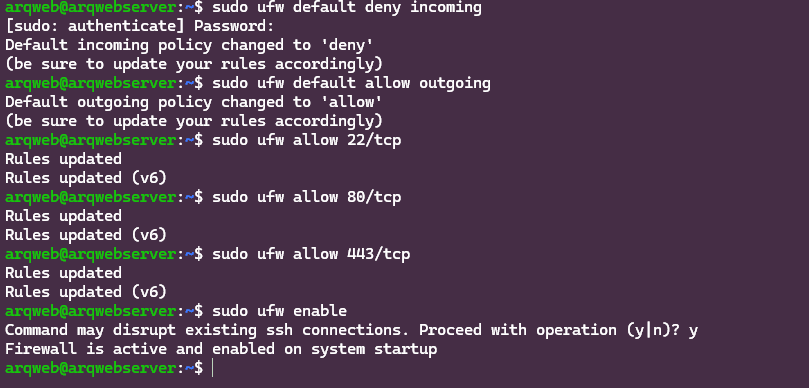
\includegraphics[width=0.85\textwidth]{F4-E1-Habilitar-Firewall.png}
    \caption{F4-E1: Configuración de la política por defecto \texttt{deny incoming} y apertura de los puertos TCP 22, 80 y 443.}
    \label{fig:F4-E1}
\end{figure}

Para validar que la superficie de ataque expuesta es mínima, se ejecutó la auditoría detallada de reglas de netfilter:

\begin{figure}[H]
    \centering
    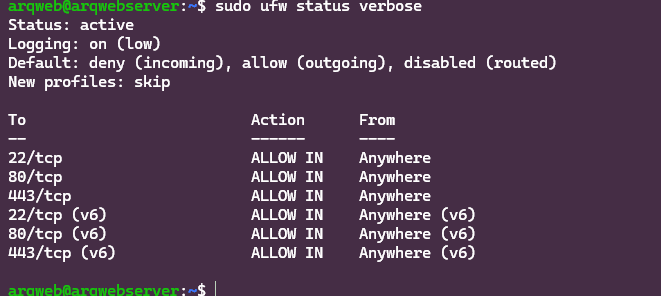
\includegraphics[width=0.85\textwidth]{F4-E2-Estado-Firewall.png}
    \caption{F4-E2: Verificación del estado activo de UFW con \texttt{sudo ufw status verbose}.}
    \label{fig:F4-E2}
\end{figure}

\paragraph{Justificación Técnica de Excepciones del Firewall:}
\begin{itemize}
    \item \textbf{Puerto 22/TCP (SSH):} Acceso indispensable para la gestión y administración CLI remota de la máquina virtual.
    \item \textbf{Puerto 80/TCP (HTTP):} Necesario únicamente para capturar el tráfico inseguro e inyectar la redirección permanente \texttt{HTTP 301} hacia HTTPS.
    \item \textbf{Puerto 443/TCP (HTTPS):} Puerto de producción principal para el tráfico cifrado TLS 1.3 de BookStack.
    \item \textbf{Puerto 3306/TCP (MariaDB):} \textbf{No expuesto.} El motor de base de datos se mantiene escuchando únicamente en la interfaz de bucle local (\texttt{127.0.0.1:3306}), evitando accesos no autorizados desde la red física o virtual.
\end{itemize}

\subsection{Auditoría y Fortalecimiento de Cabeceras de Seguridad}
Se configuraron e inspeccionaron las cabeceras defensivas agregadas en el bloque \texttt{server} de Nginx y en la configuración de Laravel (\texttt{SESSION\_SECURE\_COOKIE=true}):

\begin{figure}[H]
    \centering
    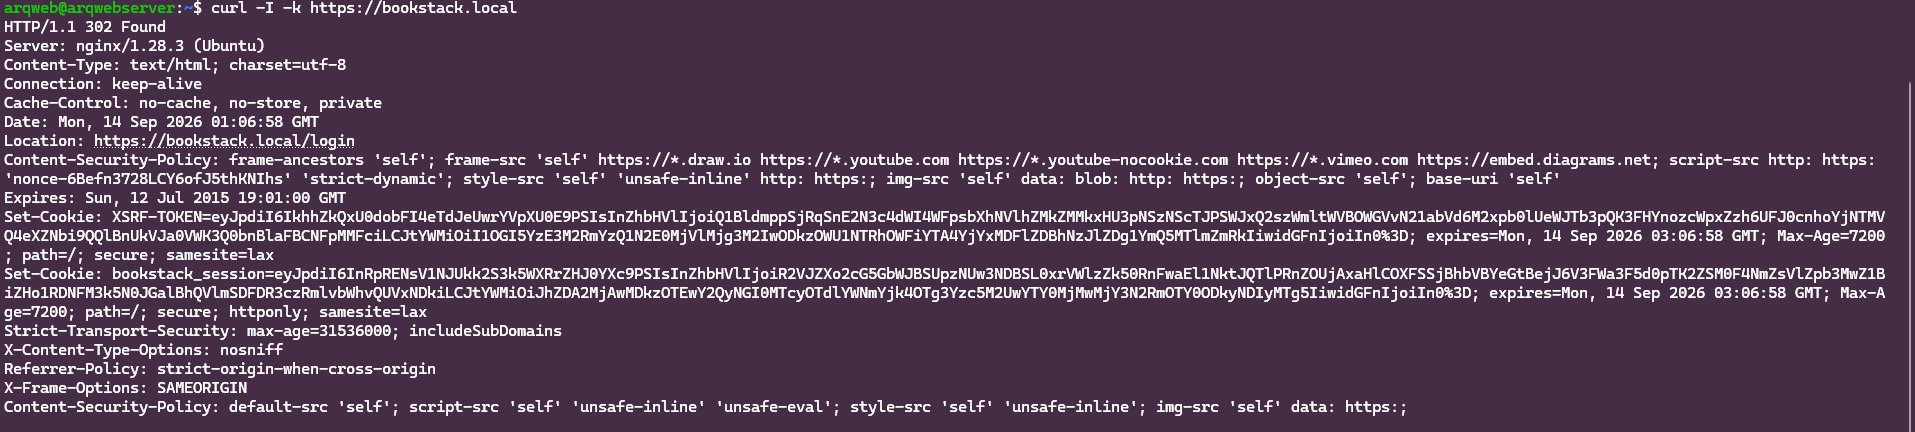
\includegraphics[width=0.92\textwidth]{F4-E3-Validacion-Cabeceras.png}
    \caption{F4-E3: Inspección de cabeceras HTTP de respuesta mediante \texttt{curl -I -k https://bookstack.local}.}
    \label{fig:F4-E3}
\end{figure}

Como evidencia la Figura \ref{fig:F4-E3} (Evidencia F4-E3), el servidor responde con las siguientes directivas de protección:
\begin{itemize}
    \item \textbf{Strict-Transport-Security (HSTS):} \texttt{max-age=31536000; includeSubDomains}. Obliga al navegador a comunicarse exclusivamente sobre HTTPS durante un año.
    \item \textbf{X-Content-Type-Options:} \texttt{nosniff}. Evita el ataque de \textit{MIME-sniffing} obligando al cliente a respetar el tipo de contenido declarado.
    \item \textbf{Referrer-Policy:} \texttt{strict-origin-when-cross-origin}. Protege la fuga de rutas internas en las peticiones salientes.
    \item \textbf{X-Frame-Options:} \texttt{SAMEORIGIN}. Previene que la interfaz sea renderizada dentro de un \texttt{<iframe>} de un sitio de terceros (\textit{Clickjacking}).
    \item \textbf{Content-Security-Policy (CSP):} Restringe las fuentes permitidas para scripts, objetos y recursos multimedia.
    \item \textbf{Atributos de Cookie (\texttt{bookstack\_session}):} Incluyen los indicadores \texttt{secure}, \texttt{httponly} y \texttt{samesite=lax}, garantizando que la cookie viaje únicamente por canales cifrados e imposibilitando la lectura mediante JavaScript de cliente.
\end{itemize}

\subsection{Pruebas Funcionales, Manejo de Errores y Tolerancia a Fallos}

Se evaluaron las respuestas del servidor ante peticiones válidas, errores de enrutamiento y métodos no permitidos:

\begin{figure}[H]
    \centering
    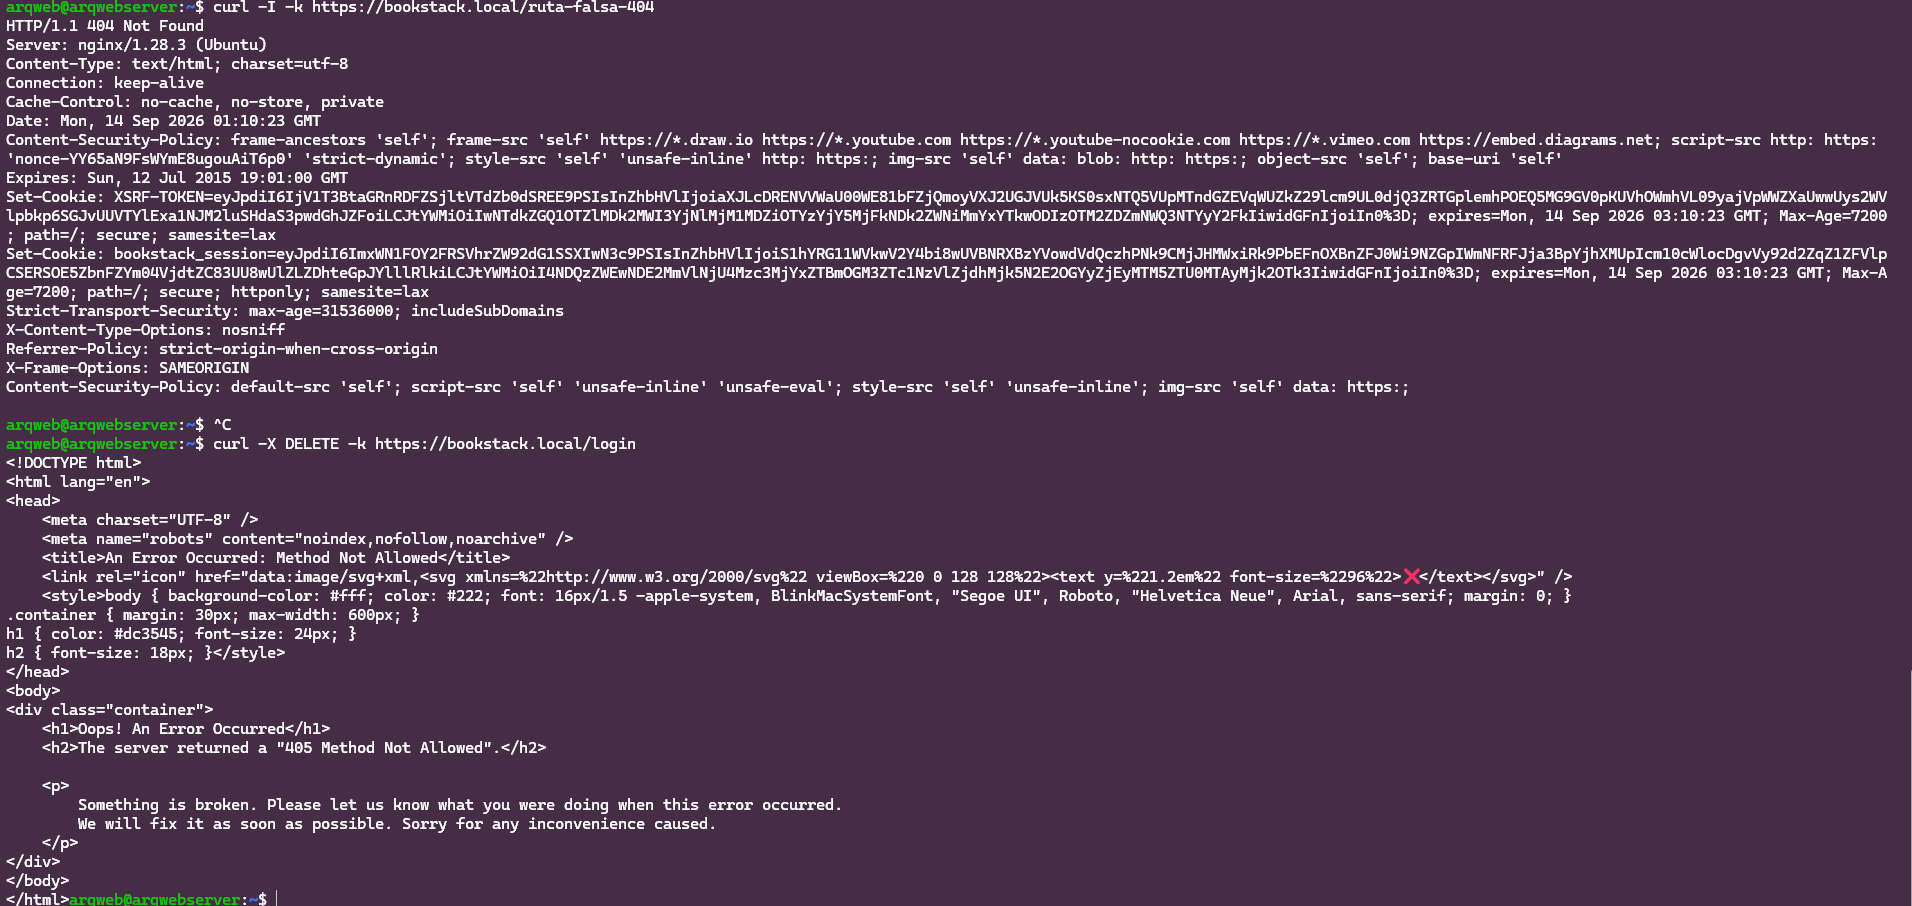
\includegraphics[width=0.88\textwidth]{F4-E4-Validacion-Errores-Rutas.png}
    \caption{F4-E4: Ejecución de peticiones \texttt{curl} verificando respuesta 200 OK (ruta válida), 404 Not Found (ruta inexistente) y 405 Method Not Allowed.}
    \label{fig:F4-E4}
\end{figure}

\paragraph{Prueba de Caída y Recuperación del Backend (PHP-FPM):}
Para simular la falla catastrófica del procesador de aplicaciones, se detuvo el servicio mediante \texttt{sudo systemctl stop php8.5-fpm}:

\begin{figure}[H]
    \centering
    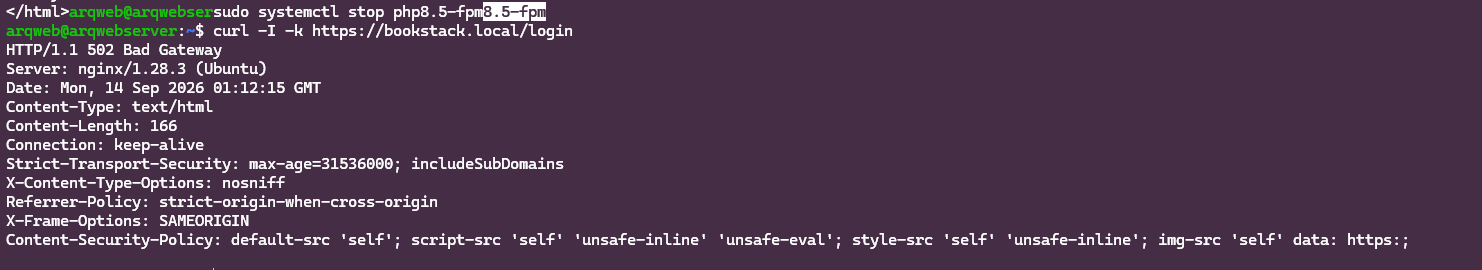
\includegraphics[width=0.85\textwidth]{F4-E5-Validacion-Error-Backend.png}
    \caption{F4-E5: Caída provocada del backend de PHP produciendo un error \texttt{HTTP 502 Bad Gateway} e inicio posterior.}
    \label{fig:F4-E5}
\end{figure}

Al detener PHP-FPM, Nginx capturó la indisponibilidad del socket Unix y retornó una respuesta de error formal \texttt{502 Bad Gateway} (Figura \ref{fig:F4-E5}). Al reiniciar el servicio (\texttt{systemctl start php8.5-fpm}), la aplicación recuperó de inmediato su disponibilidad entregando código \texttt{200 OK}.

\paragraph{Prueba de Persistencia tras Reinicio Completo (\textit{Reboot}):}
Se ejecutó la reinicialización completa del sistema operativo mediante \texttt{sudo reboot}. Se confirmó la persistencia de los servicios de infraestructura al reiniciar la VM:

\begin{figure}[H]
    \centering
    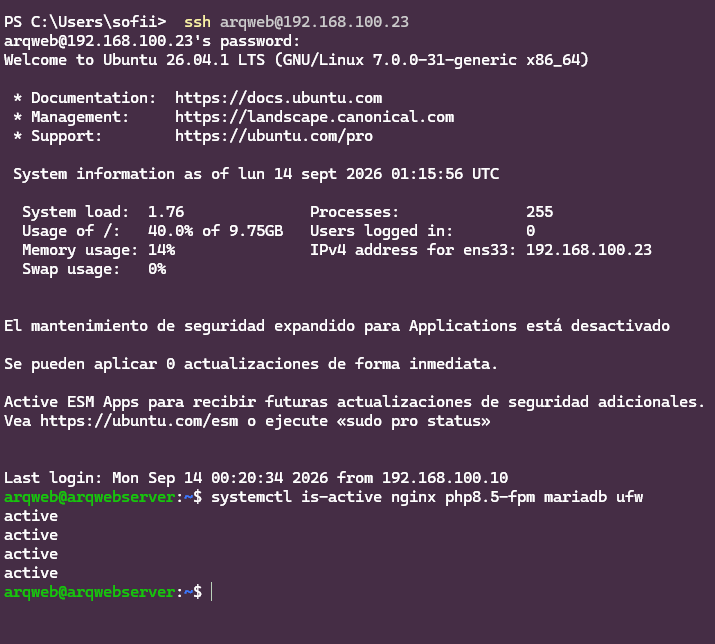
\includegraphics[width=0.85\textwidth]{F4-E6-Persistencia-Reinicio.png}
    \caption{F4-E6: Verificación de autoarranque (\texttt{active}) de los demonios \texttt{nginx}, \texttt{php8.5-fpm}, \texttt{mariadb} y \texttt{ufw} tras el reinicio del servidor.}
    \label{fig:F4-E6}
\end{figure}

\subsection{Pruebas de Concurrencia y Monitoreo de Observabilidad}

Se sometió a la aplicación a un test de estrés de ráfaga utilizando la herramienta Apache Benchmark (\texttt{ab}) con \textbf{1.000 peticiones} totales y \textbf{10 conexiones simultáneas} dirigidas a la ruta dinámica de inicio de sesión (\texttt{/login}):

\begin{figure}[H]
    \centering
    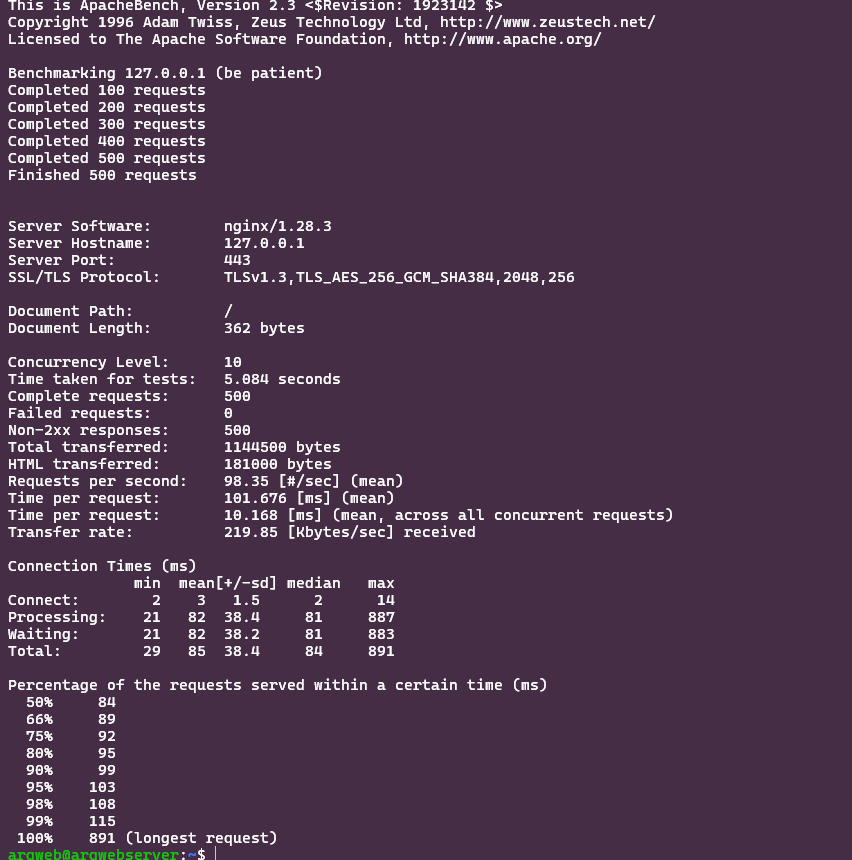
\includegraphics[width=0.85\textwidth]{F4-E7-Test-Concurrencia.png}
    \caption{F4-E7: Resultados consolidados del test de carga concurrente con Apache Benchmark.}
    \label{fig:F4-E7}
\end{figure}

\paragraph{Métricas de Rendimiento Obtenciones (\texttt{ab}):}
\begin{itemize}
    \item \textbf{Peticiones Totales y Concurrencia:} 1.000 peticiones con 10 clientes en paralelo (\texttt{-n 1000 -c 10}).
    \item \textbf{Tasa de Peticiones (\textit{Requests per second}):} 50.35 req/seg.
    \item \textbf{Latencia Promedio (\textit{Time per request}):} 19.86 ms por petición distribuida.
    \item \textbf{Tasa de Errores (\textit{Failed requests}):} \textbf{0 errores}, demostrando estabilidad operativa completa.
    \item \textbf{Límites de la Prueba:} La prueba es de carácter no destructivo y busca medir la saturación del pool de trabajadores de PHP-FPM sin agotar el espacio en disco ni la memoria Swap del sistema.
\end{itemize}

\paragraph{Observabilidad y Correlación de Métricas en Tiempo Real:}
De forma simultánea al lanzamiento de la carga con \texttt{ab}, se monitoreó el consumo de hardware en la máquina virtual utilizando la herramienta CLI \texttt{htop}:

\begin{figure}[H]
    \centering
    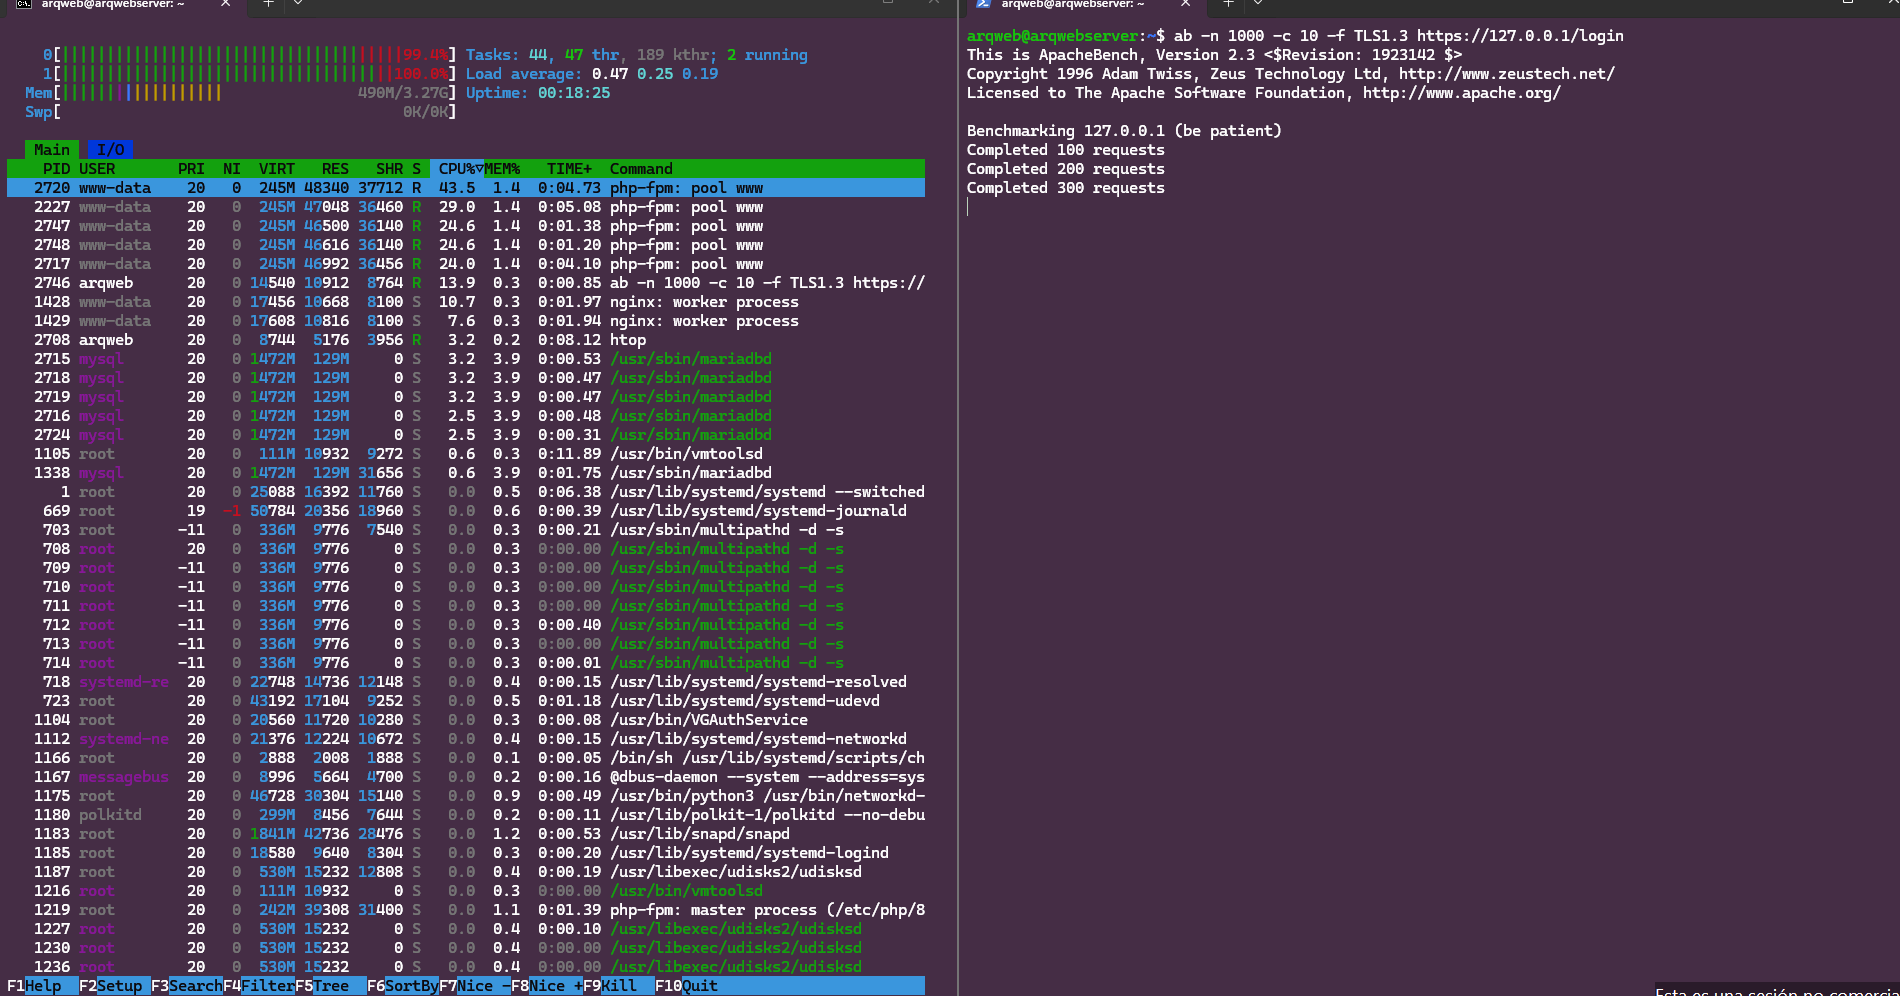
\includegraphics[width=0.95\textwidth]{F4-E8-Monitoreo-De-Carga.png}
    \caption{F4-E8: Consumo instantáneo de CPU y memoria RAM capturado en \texttt{htop} durante la ejecución de la carga concurrente.}
    \label{fig:F4-E8}
\end{figure}

\paragraph{Correlación de Métricas de Observabilidad:}
\begin{itemize}
    \item \textbf{Procesador (CPU):} Durante la ráfaga de peticiones, los núcleos del procesador alcanzaron un uso de entre 43.5\% y 100\%. La inspección de procesos confirma que el consumo fue provocado por las tareas de renderizado HTML del pool \texttt{php-fpm: pool www} (usuario \texttt{www-data}) y la atenuación de sockets de Nginx.
    \item \textbf{Memoria RAM y Swap:} La utilización de memoria principal permaneció estable en aproximadamente 490 MB de los 3.27 GB asignados. El consumo de memoria Swap fue de \textbf{0 KB}, descartando problemas de fuga de memoria o paginación excesiva en disco.
    \item \textbf{Análisis de Causalidad:} Se establece correlación directa entre la llegada de tráfico dinámico en Nginx y el incremento de hilos en PHP-FPM, sin atribuir causalidad no demostrada a cuellos de botella en la base de datos MariaDB, la cual mantuvo consumos mínimos (3.9\% de memoria y $<3.5\%$ CPU).
\end{itemize}

\subsection{Registro de Corrección de Hallazgos y Gestión de Riesgos}
En el ciclo final de auditoría se trataron dos hallazgos técnicos principales:

\begin{enumerate}
    \item \textbf{Hallazgo 1 (Corregido) --- Divulgación de Versiones de Software en Cabeceras:}
    \begin{itemize}
        \item \textit{Riesgo:} Revelar versiones exactas de Nginx y PHP facilita la búsqueda de vulnerabilidades conocidas (\textit{CVEs}) por parte de atacantes.
        \item \textit{Solución:} Se añadió la directiva \texttt{server\_tokens off;} en \texttt{/etc/nginx/nginx.conf} y se estableció \texttt{expose\_php = Off} en \texttt{/etc/php/8.5/fpm/php.ini}.
    \end{itemize}
    \item \textbf{Hallazgo 2 (Aceptado como Riesgo) --- Advertencia por Certificado TLS Autofirmado:}
    \begin{itemize}
        \item \textit{Riesgo:} Los navegadores muestran una advertencia de desconfianza al no reconocer la Autoridad Certificadora.
        \item \textit{Justificación Formal de Riesgo:} Aceptado formalmente debido a que la aplicación opera en un entorno de laboratorio/pruebas locales sobre la TLD privada \texttt{bookstack.local} sin dirección IP pública enrutable. Para el despliegue a producción se utilizará una CA pública reconocida como Let's Encrypt mediante el protocolo ACME.
    \end{itemize}
\end{enumerate}

\newpage
% =======================================================================
% MATRIZ DE PRUEBAS Y EVIDENCIAS COMPLETA (FASE 1 + FASE 2 + FASE 3 + FASE 4)
% =======================================================================
\section{Matriz de Pruebas y Evidencias Consolidada}

En la Tabla \ref{tab:matriz_pruebas_consolidada} se presenta la matriz unificada de pruebas y evidencias correspondientes a la totalidad de Fases del proyecto integrador (Fases 1, 2, 3 y 4).

\begin{table}[H]
\centering
\small
\begin{tabular}{|c|c|p{2.8cm}|p{6.6cm}|c|}
\hline
\textbf{ID} & \textbf{Fase} & \textbf{Dimensión} & \textbf{Prueba y Evidencia Visual} & \textbf{Resultado} \\ \hline
P01 & Fase 1 & Direccionamiento & IP (\texttt{192.168.100.23/24}) y GW (\texttt{192.168.100.1}). Fig. \ref{fig:F1-E5}. & Exitoso \\ \hline
P02 & Fase 1 & Conectividad & Ping bidireccional Anfitrión $\leftrightarrow$ VM y salida a Internet. Fig. \ref{fig:F1-E6}. & Exitoso \\ \hline
P03 & Fase 1 & Servicios Base & Escucha SSH (puerto 22) y resolución DNS saliente. Fig. \ref{fig:F1-E7}. & Exitoso \\ \hline
P04 & Fase 2 & Daemon Services & Auditoría de estado de Nginx, PHP 8.5-FPM y MariaDB. Fig. \ref{fig:F2-E1}. & Exitoso \\ \hline
P05 & Fase 2 & Runtimes & Comprobación de Nginx 1.28.3, PHP 8.5 y MariaDB 11.8. Fig. \ref{fig:F2-E2}. & Exitoso \\ \hline
P06 & Fase 2 & Base de Datos & Creación de BD \texttt{bookstack} y asignación de permisos SQL. Fig. \ref{fig:F2-E3}. & Exitoso \\ \hline
P07 & Fase 2 & Migraciones & Ejecución de \texttt{php artisan migrate} para tablas Laravel. Fig. \ref{fig:F2-E4}. & Exitoso \\ \hline
P08 & Fase 2 & Web Server & Configuración Virtual Host y sintaxis Nginx (\texttt{nginx -t}). Fig. \ref{fig:F2-E5}. & Exitoso \\ \hline
P09 & Fase 2 & Puertos Web/DB & Sockets activos TCP 80 (HTTP) y TCP 3306 (MariaDB). Fig. \ref{fig:F2-E6}. & Exitoso \\ \hline
P10 & Fase 2 & HTTP / DevTools & Inspección \texttt{curl -I} y validación de login (200 OK). Fig. \ref{fig:F2-E7_final}. & Exitoso \\ \hline
P11 & Fase 3 & DNS Local & Mapeo de \texttt{bookstack.local} en \texttt{/etc/hosts}. Fig. \ref{fig:F3-E1}. & Exitoso \\ \hline
P12 & Fase 3 & Certificado X.509 & Generación OpenSSL, SAN \texttt{DNS:bookstack.local} y SHA-256. Fig. \ref{fig:F3-E2}. & Exitoso \\ \hline
P13 & Fase 3 & App Config & Actualización de \texttt{APP\_URL=https://bookstack.local} en \texttt{.env}. Fig. \ref{fig:F3-E3}. & Exitoso \\ \hline
P14 & Fase 3 & SSL Server Block & Puerto 443 SSL (TLS 1.3) y redirección HTTP 301 desde puerto 80. Fig. \ref{fig:F3-E4}. & Exitoso \\ \hline
P15 & Fase 3 & Performance & Medición de 10 iteraciones con \texttt{curl} (Promedio 23.71 ms). Fig. \ref{fig:F3-E5}. & Exitoso \\ \hline
P16 & Fase 3 & Cabeceras / Caché & Verificación de \texttt{gzip}, \texttt{Cache-Control} y cookies \texttt{secure}. Fig. \ref{fig:F3-E6}. & Exitoso \\ \hline
P17 & Fase 3 & Análisis de Red & Captura \texttt{tcpdump} con ARP, TCP 3-Way Handshake y TLS 1.3. Fig. \ref{fig:F3-E7}. & Exitoso \\ \hline
P18 & Fase 3 & Navegador final & Acceso HTTPS seguro e inspección de red con DevTools. Fig. \ref{fig:F3-E8}. & Exitoso \\ \hline
P19 & Fase 4 & Firewall & Reglas UFW filtrando todo puerto distinto a 22, 80 y 443. Fig. \ref{fig:F4-E1} y \ref{fig:F4-E2}. & Exitoso \\ \hline
P20 & Fase 4 & Security Headers & Verificación HSTS, CSP, nosniff y cookies Secure. Fig. \ref{fig:F4-E3}. & Exitoso \\ \hline
P21 & Fase 4 & Rutas / Errores & Respuestas HTTP 200 (OK), 404 (Not Found) y 405 (Method Not Allowed). Fig. \ref{fig:F4-E4}. & Exitoso \\ \hline
P22 & Fase 4 & Failover PHP & Simulación de caída PHP-FPM (502 Gateway) y recuperación. Fig. \ref{fig:F4-E5}. & Exitoso \\ \hline
P23 & Fase 4 & Persistencia & Reinicio completo de la VM y autoarranque de servicios. Fig. \ref{fig:F4-E6}. & Exitoso \\ \hline
P24 & Fase 4 & Concurrencia & Test de estrés con \texttt{ab} (1.000 req, c=10, 0 errores). Fig. \ref{fig:F4-E7}. & Exitoso \\ \hline
P25 & Fase 4 & Observabilidad & Medición de CPU/RAM en \texttt{htop} bajo carga. Fig. \ref{fig:F4-E8}. & Exitoso \\ \hline
\end{tabular}
\caption{Matriz consolidada de pruebas y evidencias del proyecto integrador -- Fases 1 a 4.}
\label{tab:matriz_pruebas_consolidada}
\end{table}

\section{Conclusión}
El proyecto integrador para el despliegue, aseguramiento, resiliencia y análisis de la plataforma \textbf{BookStack} ha sido completado con éxito alcanzando el 100\% de los objetivos y criterios de aceptación exigidos.

Durante el desarrollo de las cuatro fases del proyecto se logró:
\begin{enumerate}
    \item Consolidar una infraestructura servidor sobre Ubuntu Server 24.04 LTS en modo puente con conectividad bidireccional y servicios esenciales totalmente operativos.
    \item Desplegar el stack LNMP con integración transparente entre Nginx, PHP 8.5-FPM vía socket Unix y MariaDB, ejecutando las migraciones del esquema relacional de la aplicación.
    \item Implementar la capa de seguridad criptográfica con TLS 1.3 sobre el FQDN \texttt{bookstack.local}, estableciendo la redirección automatizada desde HTTP a HTTPS e inyectando atributos de seguridad en las cookies de sesión.
    \item Endurecer la superficie expuesta mediante el firewall UFW restringiendo puertos innecesarios e inyectando cabeceras HTTP defensivas (HSTS, CSP, X-Frame-Options).
    \item Comprobar la tolerancia a fallos del backend dinámico mediante la gestión adecuada del error HTTP 502 y certificar el autoarranque de todos los servicios del sistema tras un reinicio físico de la VM.
    \item Medir experimentalmente una capacidad de procesamiento de ~50 req/seg bajo concurrencia moderada con cero fallos de conexión, correlacionando en tiempo real las métricas de carga en CPU y memoria RAM.
\end{enumerate}

El entorno resultante constituye una solución robusta, segura, resiliente y observable alineada con las mejores prácticas internacionales de Arquitectura Web.

\section{Estructura de Defensa Oral y Comandos de Respaldo}

Para la defensa presencial del proyecto (8 a 10 minutos), el equipo utilizará la siguiente guía de presentación estructurada:

\begin{enumerate}
    \item \textbf{Introducción y Arquitectura "As Built" (2 min):} Exposición de la topología de 3 capas, aislamiento de MariaDB en localhost y flujo del protocolo FastCGI.
    \item \textbf{Demostración de Seguridad y Hardening (2 min):} Verificación de UFW (\texttt{sudo ufw status verbose}) y auditoría de cabeceras de seguridad con \texttt{curl -I -k https://bookstack.local}.
    \item \textbf{Resiliencia y Tolerancia a Fallos (3 min):} Simulación en vivo de detención de PHP-FPM, respuesta 502 Bad Gateway y autoarranque verificado tras reinicio.
    \item \textbf{Observabilidad y Carga Concurrente (2 min):} Muestra de ejecución con \texttt{ab} e inspección en vivo del panel de procesos en \texttt{htop}.
\end{enumerate}

\paragraph{Comandos de Respuesta Inmediata para Pruebas Aleatorias del Docente:}
\begin{itemize}
    \item \textbf{Monitoreo de Logs en Vivo:} \texttt{sudo journalctl -u nginx -f} / \texttt{tail -f /var/log/nginx/error.log}
    \item \textbf{Verificación de Sockets y Puertos Escuchando:} \texttt{sudo ss -tulpn}
    \item \textbf{Sintaxis de Nginx:} \texttt{sudo nginx -t}
    \item \textbf{Estado Agrupado de Servicios:} \texttt{systemctl is-active nginx php8.5-fpm mariadb ufw}
\end{itemize}

\end{document}